\documentclass[10pt,a4paper]{article}
\usepackage[margin=1in]{geometry}
\usepackage{amsmath,amssymb}
\usepackage{graphicx}
\usepackage{booktabs}
\usepackage{longtable}
\usepackage{hyperref}
\usepackage{xcolor}
\usepackage{authblk}
% NOTE: written for the standard article class so it compiles without
% extra style files. Swap to IEEEtran / your target venue's class if
% you have it installed; the content and equations are class-agnostic.

% ==============================================================
% AUTHOR NOTE (READ BEFORE COMPILING)
% ------------------------------------------------------------
% This file was generated under a strict "code-is-the-only-source-of-truth"
% rule. Every equation below is annotated with a CODE TRACE comment
% pointing to the exact file/function/variables it was derived from.
% Anywhere the implementation does not define a value, a
% [NOT PRESENT IN CODE -- AUTHOR INPUT REQUIRED] marker is used instead
% of an invented number. Do not delete these markers without replacing
% them with a value you have verified against actual code output.
% ==============================================================

\begin{document}

\title{An Integrated LMCI-MCLP Framework for Last-Mile Connectivity Assessment and Intervention Prioritization: \\
A Case Study of the Hyderabad Metro}

\author{Pansuriya Foram Rasikbhai \\ \small [AUTHOR INPUT REQUIRED: affiliation, department, institution, contact]}
\date{}

\maketitle

% ==============================================================

\begin{abstract}
Urban metro systems in rapidly growing Indian cities face a persistent challenge: ensuring equitable access to stations through reliable last-mile connectivity. This paper presents an integrated framework that combines a Last-Mile Connectivity Index (LMCI) with a Maximal Covering Location Problem (MCLP) model to assess accessibility and prioritise interventions across the Hyderabad Metro network. Using multimodal GTFS data from metro, bus, suburban rail, and feeder services, we construct a spatial-temporal accessibility score incorporating route diversity, temporal frequency across morning, midday, and evening windows, and walk-zone accessibility. Entropy weighting derives objective component weights, and an equity-sensitive priority score combines LMCI deficit, demand signals from business POIs and schools, persistence of transit deserts, and temporal gaps. The analysis of 57 metro stations reveals 40 persistent transit deserts (70\% of the network) and six high-demand - low-service stations, with S. R. Nagar emerging as the highest-priority intervention target (priority index = 10.0). A greedy MCLP algorithm identifies five strategic intervention locations that collectively achieve 8.61\% weighted demand coverage, with coverage increasing to 13.53\% at k=10. Scenario simulations demonstrate that integrated multimodal hubs yield the greatest modelled accessibility gains (mean impact score = 1.94), followed by feeder shuttle integration (1.61) and bus frequency enhancement (1.25). The framework provides transit agencies with a reproducible, explainable, and equity-aware decision-support tool for evidence-based infrastructure investment. All code and intermediate outputs are published to ensure full reproducibility.

\keywords{Last-mile connectivity, LMCI, MCLP, transit deserts, transportation equity, GTFS, Hyderabad Metro}
\end{abstract}

% ==============================================================
% DATA AND CODE AVAILABILITY
% ==============================================================
The complete source code and input data are available at
\href{https://github.com/pansuriyaForam/hyderabad-metro-last-mile-intelligence}{github.com/pansuriyaForam/hyderabad-metro-last-mile-intelligence}
(Data directory:
\href{https://github.com/pansuriyaForam/hyderabad-metro-last-mile-intelligence/tree/main/Data}{github.com/.../tree/main/Data}).

% ==============================================================
\section{Introduction}

Urban transportation networks in India face a critical challenge: the first-mile and last-mile connectivity problem. While major cities have invested heavily in high-capacity metro rail systems, the accessibility of these networks remains uneven, especially in peripheral and economically disadvantaged areas. Rapid urbanisation, informal settlement patterns, and insufficient feeder service coordination create transit desert zones where residents lack feasible multimodal access to transit hubs \cite{Karner2025,Wang2024}. This spatial inequality undermines the equity and sustainability goals of public transportation agencies.

The Hyderabad Metro Rail Limited (HMRL) system, operational since 2017, provides 69 km of service across the metropolitan region. However, a systematic assessment of last-mile connectivity across the network has been lacking. Most transit accessibility studies in Indian cities rely on simple distance-based metrics (e.g., 400 m or 800 m buffer zones) without considering multimodal integration, temporal frequency variability, or demand heterogeneity \cite{Rathod2019,Umair2025,Ghosh2025}. Furthermore, the temporal aspect of accessibility—specifically, how service quality changes during peak and off-peak hours—remains underexplored despite its importance for equity and mode choice \cite{TravelTime2023}. The availability of open General Transit Feed Specification (GTFS) data has enabled new approaches to accessibility analysis \cite{Malaysia2025,Pourramazani2026}, yet systematic frameworks that combine multimodal stop density, temporal frequency, and demand signals remain scarce in the Indian context.

This paper addresses these gaps by developing an integrated Last-Mile Connectivity Index (LMCI) and Maximal Covering Location Problem (MCLP) optimisation framework. The LMCI combines multimodal stop density (weighted by route diversity), temporal transit frequency extracted from GTFS schedules across morning, midday, and evening windows, and walk-zone accessibility into a composite score \cite{Rathod2025a}. Entropy weighting is applied to derive objective component weights, ensuring that the relative importance of each accessibility dimension is determined by the data itself rather than by arbitrary assumptions. The MCLP algorithm, implemented as a greedy approximation \cite{Church1974}, identifies strategic locations for intervention to maximise weighted demand coverage within resource limits \cite{Equity2020}. We incorporate equity-weighted priority scoring that balances LMCI deficit, demand signals from business POIs and affordable schools, persistence of transit deserts across temporal windows, and temporal gaps \cite{Cha2008,Jiao2023}. This equity-sensitive formulation ensures that persistently underserved stations receive explicit policy priority, addressing a key limitation of coverage-maximising approaches that may inadvertently favour already well-served areas.

The analysis covers 57 metro stations and reveals 40 persistent transit deserts (70\% of the network), with S. R. Nagar emerging as the highest-priority intervention target (priority index = 10.0). Demand-service mismatch analysis identifies six critical high-demand--low-service stations requiring immediate attention. The MCLP optimisation demonstrates that five strategically selected intervention locations achieve 8.61\% weighted demand coverage, with coverage increasing to 13.53\% at \(k=10\). Scenario simulations of five intervention types—integrated multimodal hubs, feeder shuttle integration, bus frequency enhancement, e-rickshaw last-mile loops, and pedestrian access upgrades—show that integrated multimodal hubs yield the greatest modelled accessibility gains (mean impact score = 1.94), followed by feeder shuttles (1.61) and frequency enhancements (1.25).

Our contributions are threefold: (1) a deterministic, fully explainable, and reproducible accessibility framework validated against GTFS data completeness and demand signal quality, with all code and intermediate outputs publicly available; (2) identification of 40 persistent transit deserts and prioritised intervention sites—S. R. Nagar, Miyapur, Ameerpet, Rasoolpura, and Kukatpally—using entropy-weighted composite scoring; and (3) scenario simulations demonstrating that integrated multimodal hubs provide the greatest modelled accessibility improvements, offering evidence-based guidance for infrastructure investment planning.

The remainder of this paper is organised as follows. Section~\ref{sec:data} describes the study area and data sources. Section~\ref{sec:methodology} presents the LMCI formulation, entropy weighting, MCLP optimisation, equity-weighted priority scoring, and intervention scenario simulation. Section~\ref{sec:results} reports the empirical findings. Section~\ref{sec:discussion} interprets the results and discusses policy implications. Section~\ref{sec:limitations} acknowledges the study's limitations, and Section~\ref{sec:conclusion} concludes the paper.

% ==============================================================

\section{Literature Review}

Recent advances in transportation equity research emphasise that accessibility extends beyond mere distance, involving multiple dimensions \cite{Karner2025}. Karner et al. pointed out key issues in measuring equity: reliance on binary thresholds (e.g., ``within 800 m or not''), ignoring variations in service frequency, and overlooking temporal accessibility aspects. Using composite indices that consider density, frequency, and connectivity, such as the Public Transport Accessibility Level (PTAL), which provides more detailed assessments \cite{Rathod2019}. PTAL converts walking distance and frequency into a scale ranging from 0 to 6; Rathod et al. modified this approach for Indian cities, discovering that evaluations based on PTAL highlight accessibility inequalities that methods focusing solely on distance overlook \cite{Rathod2019,Rathod2025a}.

The challenge of last-mile connectivity in transportation is regarded as a facility location optimisation challenge. The Maximal Covering Location Problem (MCLP), introduced by Church and ReVelle, aims to choose $k$ facilities that maximise the coverage of demand within a specified service radius \cite{Church1974}. MCLP has found extensive application in areas such as healthcare, emergency response, and transit planning, but its use in Indian cities remains limited. Cha demonstrated that MCLP can enhance equity by focusing on underserved populations \cite{Cha2008}. Recent adaptations have included equity weights \cite{Equity2020} and multi-objective formulations \cite{MultiObjective2023}, although these can be computationally intensive for large metropolitan networks.

As transit agencies around the world release open GTFS data, the analysis of accessibility based on GTFS is becoming increasingly popular \cite{Pourramazani2026,Malaysia2025}. Wang and Loo established a framework to recognise populations that are ``transit disadvantaged,'' distinguishing between geographic isolation and challenges related to temporal accessibility \cite{Wang2024}. In India, the use of GTFS for analysis is still in its infancy since many transit agencies do not publish GTFS feeds, and aspects such as demand signals (points of interest, or school weighting) are managed informally. Research on last-mile access in India primarily concentrates on first-mile access (walking or cycling to transit), creating a void in the understanding of last-mile access (from transit to the final destination), which this study aims to fill \cite{Umair2025,Ghosh2025,Wani2026}.

Ghosh et al. found that both accessibility and affordability influence transit ridership in Indian metro cities, with interventions targeting only one having a limited effect \cite{Ghosh2025}. Similarly, Umair et al. identified feeder shuttles and e-rickshaw loops as cost-effective last-mile solutions in New Delhi \cite{Umair2025}. However, these lack systematic prioritisation frameworks. This paper proposes an integrated LMCI-MCLP simulation approach that combines demand analysis, coverage optimisation, and scenario testing to fill this research gap.

% ------------------------------------------------------------

\section{Study Area and Data}
% CODE-DERIVED DATA DESCRIPTION

The study area is constrained to a fixed geographic bounding box defined
in the preprocessing configuration.

% ------------------------------------------------------------
% CODE TRACE
% Source: preprocessing.py
% Class: Config
% Variables: bbox_lat_min, bbox_lat_max, bbox_lon_min, bbox_lon_max
% ------------------------------------------------------------
The bounding box used to filter all stop and demand records is
$\text{lat} \in [16.8,\,17.8]$, $\text{lon} \in [77.5,\,79.5]$
(\texttt{preprocessing.py}, \texttt{Config}). The same bounding box is
independently redeclared in \texttt{lmci.py} (\texttt{LMCIConfig}) with
identical numeric values.

\subsection{Data Sources}
Data are ingested from GTFS-formatted transit feeds and two GeoJSON
demand layers:
\begin{itemize}
\item \textbf{HMRL} (Hyderabad Metro Rail) - \texttt{stops.txt} only
  (\texttt{preprocessing.py}, \texttt{GTFSLoader.HMRL\_FILES}).
\item \textbf{TGSRTC} (bus) - \texttt{stops.txt}, \texttt{stop\_times.txt},
  \texttt{trips.txt}, \texttt{routes.txt} (\texttt{TGSRTC\_FILES}; only
  \texttt{stops.txt} and \texttt{stop\_times.txt} are required, \texttt{trips.txt}
  is optional and used only for route-diversity joins).
\item \textbf{MMTS} (suburban rail) - \texttt{stops.txt}, \texttt{stop\_times.txt}
  (optional feed, loaded in \texttt{lmci.py}).
\item \textbf{Feeder} services - \texttt{stops.txt}, \texttt{stop\_times.txt},
  \texttt{frequencies.txt} (optional feed).
\item Demand layers: \texttt{data/external/poi\_business.geojson} and
  \texttt{data/external/Affordable\_Schools.geojson}
  (\texttt{preprocessing.py}, \texttt{Config.poi\_path}, \texttt{Config.school\_path}).
\end{itemize}

\subsection{Coordinate Reference Systems}
% CODE TRACE
% Source: preprocessing.py (Config.wgs84_crs, Config.metric_crs)
%         lmci.py (LMCIConfig.wgs84_crs, LMCIConfig.utm_crs)
%         mclp.py (MCLPConfig.wgs84_crs, MCLPConfig.metric_crs)
%         scoring.py (ScoringConfig.wgs84_crs, ScoringConfig.metric_crs)
%         simulation.py (SimulationConfig.wgs84_crs, SimulationConfig.metric_crs)
All modules use WGS84 (EPSG:4326) for storage/exchange and UTM Zone 44N
(EPSG:32644) for metric distance computation. Both values are
redeclared independently and identically in every configuration class
listed above.

\subsection{Metro Station Filtering}
% CODE TRACE
% Source: preprocessing.py
% Function: GTFSLoader.load_metro_stops()
Only GTFS \texttt{location\_type = 1} records are retained as parent
stations; \texttt{location\_type = 0} platform records are dropped.
Station names containing the substrings \texttt{"Arm"}, \texttt{"Lift"},
\texttt{"Escalator"}, or \texttt{"Staircase"} (case-insensitive regex) are
removed as non-station infrastructure. Records are then bounding-box
filtered and de-duplicated on \texttt{stop\_id}.

\subsection{Demand Point Construction}
% CODE TRACE
% Source: preprocessing.py
% Functions: extract_latlon(), load_demand_points(), filter_demand_within_metro_corridor()
Demand points are the union of business POIs and affordable-school
locations, each tagged with a \texttt{type} column (\texttt{"business"} /
\texttt{"school"}). After null- and bounding-box filtering and exact
duplicate removal on \texttt{(lat, lon, type)}, demand points are
restricted to the \emph{Metro Influence Corridor} - the union of
circular buffers of radius \texttt{metro\_influence\_corridor\_m = 3000.0}
metres around every metro station
(\texttt{preprocessing.py}, \texttt{Config.metro\_influence\_corridor\_m},
function \texttt{filter\_demand\_within\_metro\_corridor()}). Buffering
and the point-in-polygon test are performed in EPSG:32644.

% THEORY NOTE - AUTHOR TO DEVELOP
% Why restricting demand to a metro-influence corridor is a defensible
% choice for last-mile accessibility studies, and what its limitation is
% (it structurally cannot detect demand that is currently unserved
% because it lies entirely outside any station's 3 km buffer).

\begin{table}[h]
\centering
\caption{Study-area configuration parameters (Section~\ref{sec:params} gives the full parameter table).}
\begin{tabular}{ll}
\toprule
Parameter & Value \\
\midrule
Metro influence corridor radius & 3000.0 m \\
BBox latitude range & [16.8, 17.8] \\
BBox longitude range & [77.5, 79.5] \\
WGS84 CRS & EPSG:4326 \\
Metric/UTM CRS & EPSG:32644 \\
\bottomrule
\end{tabular}
\end{table}

% ==============================================================
\section{Methodology}

\subsection{Data Preprocessing}

\subsubsection{Min–Max Normalization}
% ------------------------------------------------------------
% CODE TRACE
% Source: preprocessing.py
% Function: minmax_norm()
% Variables: series, s.max(), s.min()
% ------------------------------------------------------------
For a numeric series $x$ of length $n$:
\begin{equation}
\hat{x}_i =
\begin{cases}
0 & \text{if } \max(x) = \min(x) \\[4pt]
\dfrac{x_i - \min(x)}{\max(x) - \min(x)} & \text{otherwise}
\end{cases}
\label{eq:minmax}
\end{equation}
This exact function (\texttt{minmax\_norm}) is imported and reused,
unmodified, by \texttt{lmci.py}, \texttt{mclp.py}, and
\texttt{simulation.py}. It is the only normalization operation present
anywhere in the six files - no z-score, robust scaling, or log
transform is implemented.

\subsubsection{Distance Calculations}
Three distinct distance computations exist in the codebase; they must
not be conflated.

\textbf{(a) Haversine distance} - \texttt{preprocessing.py},
function \texttt{haversine\_matrix()}, using
$R = 6{,}371{,}000.0$ m:
% CODE TRACE
% Source: preprocessing.py
% Function: haversine_matrix()
% Variables: lat_a, lon_a, lat_b, lon_b, EARTH_RADIUS_M
\begin{equation}
d_{ij} = 2R \arcsin\!\left(\sqrt{
\sin^2\!\frac{\Delta\varphi}{2} + \cos\varphi_i \cos\varphi_j \sin^2\!\frac{\Delta\lambda}{2}
}\right)
\label{eq:haversine}
\end{equation}
\textbf{CODE OBSERVATION:} \texttt{haversine\_matrix()} is defined but
never called by any of the other five modules. It does not participate
in the LMCI, MCLP, scoring, or simulation computations.
\textbf{AUTHOR DECISION REQUIRED:} either remove this claim from the
methodology entirely, or state explicitly that Equation~\ref{eq:haversine}
is unused dead code, not part of the reported pipeline.

\textbf{(b) Projected Euclidean distance} - computed after
reprojecting points to EPSG:32644 (\texttt{to\_gdf()},
\texttt{crs\_out=metric\_crs}/\texttt{utm\_crs}), then queried via
\texttt{scipy.spatial.cKDTree}. Used in:
\begin{itemize}
\item \texttt{lmci.py}, \texttt{build\_multimodal\_graph()} - nearest-metro
  assignment for bus/feeder/MMTS stops.
\item \texttt{lmci.py}, \texttt{attach\_demand\_counts()} - demand-point
  counting around stations.
\item \texttt{mclp.py}, \texttt{build\_coverage\_matrix()} - station-to-demand
  coverage.
\end{itemize}

\textbf{(c) Network-distance approximation via detour factor} - network
distance is never computed on an actual street/transit graph; it is a
constant multiplicative inflation of Euclidean distance.
% CODE TRACE
% Source: lmci.py, function build_multimodal_graph(); mclp.py, function build_coverage_matrix()
% Variables: dist_euclidean, detour_factor, dist_network / distance_matrix_m
\begin{equation}
d_{\text{network}} = d_{\text{euclidean}} \times \texttt{detour\_factor}
\label{eq:detour}
\end{equation}
with \texttt{detour\_factor = 1.35} (\texttt{LMCIConfig.detour\_factor},
\texttt{MCLPConfig.detour\_factor} - declared identically in both
configs). In \texttt{mclp.py} the same relationship is applied inversely
to convert a network-distance coverage radius into an equivalent
Euclidean query radius:
\begin{equation}
r_{\text{euclidean}} = \frac{\texttt{coverage\_radius\_m}}{\texttt{detour\_factor}}
\label{eq:detour_inverse}
\end{equation}
(\texttt{mclp.py}, \texttt{build\_coverage\_matrix()}). No shortest-path,
Dijkstra, or network-routing computation exists anywhere in the six
files.

\subsection{Spatial Representation: Multimodal Graph}
% ------------------------------------------------------------
% CODE TRACE
% Source: lmci.py
% Function: build_multimodal_graph()
% Variables: walk_radius_m, feeder_radius_m, detour_factor, route_diversity,
%            feeder_mode_weight, mmts_mode_weight, in_walk_zone, in_feeder_zone
% ------------------------------------------------------------
Every bus, feeder, and MMTS stop is assigned to its nearest metro
station using a $k$-d tree nearest-neighbour query on projected
coordinates. Two Boolean zone memberships are derived from
Equation~\ref{eq:detour}:
\begin{align}
\texttt{in\_walk\_zone} &= (d_{\text{network}} \le \texttt{walk\_radius\_m}) \\
\texttt{in\_feeder\_zone} &= (d_{\text{network}} \le \texttt{feeder\_radius\_m})
\end{align}
with \texttt{walk\_radius\_m = 800.0} m and
\texttt{feeder\_radius\_m = 3000.0} m (\texttt{LMCIConfig}).

\subsubsection{Route Diversity}
% CODE TRACE
% Source: lmci.py, Function: compute_route_diversity()
Route diversity is the count of unique \texttt{route\_id} values serving
a stop, computed by a four-tier fallback strategy: (A) direct
\texttt{route\_id} column in \texttt{stop\_times}; (B) join of
\texttt{stop\_times} to \texttt{trips.txt} on \texttt{trip\_id} to
recover \texttt{route\_id}; (C) a \texttt{trip\_id} string-prefix proxy
(\texttt{split("\_")[0]}); (D) a neutral fallback value of 1. The result
is clipped to a minimum of 1. Feeder-stop route diversity is scaled by
\texttt{feeder\_mode\_weight = 1.5}; MMTS stops are assigned a constant
route-diversity value equal to \texttt{mmts\_mode\_weight = 1.3}
(not computed from GTFS route counts for MMTS).
\textbf{CODE OBSERVATION:} MMTS route diversity is a fixed configuration
constant, not derived from data, while bus and feeder route diversity
are data-derived. \textbf{AUTHOR DECISION REQUIRED:} disclose this
asymmetry explicitly if MMTS stations are present in the final dataset.

\subsection{Temporal Service Characterization}
% ------------------------------------------------------------
% CODE TRACE
% Source: lmci.py
% Function: compute_temporal_frequency(), parse_gtfs_time()
% Variables: time_windows, dep_hr, trip_id, stop_id
% ------------------------------------------------------------
Three fixed time windows are hard-coded in \texttt{LMCIConfig.time\_windows}:
\begin{center}
\begin{tabular}{lll}
\toprule
Label & Start (h) & End (h) \\
\midrule
Morning & 7.0 & 10.0 \\
Midday & 11.0 & 14.0 \\
Evening & 17.0 & 21.0 \\
\bottomrule
\end{tabular}
\end{center}
GTFS \texttt{HH:MM:SS} times (including values $>24$:00:00) are parsed
to fractional hours: $t = h + m/60 + s/3600$
(\texttt{parse\_gtfs\_time()}). For each window $[t_0, t_1]$ and stop:
\begin{equation}
f_{\text{stop}} = \frac{\left|\{\text{unique trip\_id departing in } [t_0,t_1]\}\right|}{t_1 - t_0}
\label{eq:freq}
\end{equation}
(\texttt{compute\_temporal\_frequency()}), i.e. trips per hour. Feeder
frequency uses a separate headway-based computation when
\texttt{frequencies.txt} is available:
% CODE TRACE
% Source: lmci.py, Function: compute_feeder_frequency_from_headways()
\begin{equation}
\text{trips\_per\_hr} = \frac{3600}{\max(\texttt{headway\_secs},\,60)}
\label{eq:headway}
\end{equation}
averaged over all headway intervals overlapping the window. If
\texttt{frequencies.txt} is absent or produces an all-zero result for
stops that have feeder service, the pipeline falls back to computing
feeder frequency directly from \texttt{stop\_times.txt} using
Equation~\ref{eq:freq} (\texttt{attach\_temporal\_frequencies()}).

\subsubsection{MMTS Transfer Penalty}
% CODE TRACE
% Source: lmci.py, Function: compute_mmts_transfer_penalty_factor(), compute_mmts_schedule_overlap()
% Parameters: mmts_transfer_penalty_min=5.0, mmts_schedule_overlap_min=30.0, mmts_xfer_dist_m=1500.0
MMTS frequency is discounted by a transfer-penalty factor and gated by
schedule overlap:
\begin{equation}
p = \min\!\left(\frac{\texttt{mmts\_transfer\_penalty\_min}}{\max(\,(t_1-t_0)\cdot 30,\ 10^{-9}\,)},\ 0.30\right)
\label{eq:mmts_penalty}
\end{equation}
\begin{equation}
f'_{\text{mmts}} = f_{\text{mmts}} \times (1 - p)
\end{equation}
with \texttt{mmts\_transfer\_penalty\_min = 5.0} minutes and a hard cap
of $0.30$ (30\%) on the penalty. MMTS stops whose \texttt{departure\_time}
does not fall within $[t_0 - \tau,\ t_1 + \tau]$, $\tau = \texttt{mmts\_schedule\_overlap\_min}/60 = 0.5$ h,
are set to zero frequency for that window (\texttt{compute\_mmts\_schedule\_overlap()}).
A separate parameter \texttt{mmts\_xfer\_dist\_m = 1500.0} m governs
MMTS-to-metro transfer eligibility used elsewhere in
\texttt{build\_multimodal\_graph()}.

% THEORY NOTE - AUTHOR TO DEVELOP
% Explain conceptually why temporal (peak/off-peak) accessibility differs
% from a single static accessibility snapshot, and why last-mile
% connectivity is time-of-day dependent for feeder/bus-dependent trips.

\subsection{Entropy Weighting}
% ------------------------------------------------------------
% CODE TRACE
% Source: lmci.py
% Function: compute_entropy_weights()
% Input: indicator_matrix (n_samples x n_indicators), already min-max normalized
% Output: weight vector summing to 1.0
% ------------------------------------------------------------
Given a normalized indicator matrix $X \in [0,1]^{n \times m}$
(NaN/Inf replaced with 0 via \texttt{np.nan\_to\_num}):
\begin{align}
p_{ij} &= \frac{X_{ij}}{\sum_{i} X_{ij}} \quad \text{(column sums; 0 replaced by 1 to avoid division by zero)}\\
e_j &= -k \sum_{i} p_{ij}\ln p_{ij}, \quad k = \frac{1}{\ln n} \ \text{(} k=0 \text{ if } n \le 1\text{)} \\
g_j &= \max(0,\ 1 - e_j) \\
w_j &= \frac{g_j}{\sum_j g_j}
\end{align}
Special cases implemented in code: if $n=0$, all weights are set to
$1/m$; if $\sum_j g_j \le 10^{-12}$, all weights are also set to $1/m$.
No logarithm base other than natural log ($\ln$, \texttt{np.log}) is
used anywhere in the entropy computation.

\textbf{CODE OBSERVATION - three separate entropy-weighting processes
exist and must not be merged:}
\begin{enumerate}
\item \textbf{Temporal LMCI weights} - computed once from a global
matrix stacking \texttt{[density\_norm, \{window\}\_freq\_norm,
walkzone\_norm]} across every station \emph{and} every time window
(\texttt{compute\_temporal\_lmci()}), producing
$(w_{\text{density}}, w_{\text{frequency}}, w_{\text{walkzone}})$, reused
unchanged for all three window-specific LMCI values.
\item \textbf{Demand-augmented LMCI weights} - computed separately from
\texttt{[density\_norm, Morning\_freq\_norm, walkzone\_norm,
demand\_norm]} (\texttt{compute\_demand\_augmented\_lmci()}), producing
an independent $(w_{\text{density}}, w_{\text{frequency}},
w_{\text{walkzone}}, w_{\text{demand}})$ vector.
\item \textbf{Priority-index weights} - computed separately again from
\texttt{[LMCI\_Deficit, Demand, Persistence, TemporalGap]}
(\texttt{classify\_transit\_deserts()}), producing
$(w_{\text{deficit}}, w_{\text{demand}}, w_{\text{persistence}}, w_{\text{gap}})$.
\end{enumerate}
These three weight vectors are numerically independent; none is derived
from another.

\subsection{Last-Mile Connectivity Index (LMCI)}
Three distinct LMCI formulations exist in \texttt{lmci.py} and are kept
separate below, per source function.

\subsubsection{Density, Walk-Zone, and Frequency Inputs}
% CODE TRACE
% Source: lmci.py, Function: compute_temporal_lmci()
% Variables: stop_count_3km, stop_count_800m, density_norm, walkzone_norm,
%            avg_{label}_freq, {label}_freq_norm
\begin{align}
\texttt{stop\_count\_3km}_s &= \sum_{j \in \text{feeder\_zone}(s)} \texttt{route\_diversity}_j \\
\texttt{stop\_count\_800m}_s &= \left|\{\, j \in \text{feeder\_zone}(s) : \texttt{in\_walk\_zone}_j \,\}\right| \\
\texttt{density\_norm} &= \text{minmax}(\texttt{stop\_count\_3km}) \quad \text{[Eq.~\ref{eq:minmax}]}\\
\texttt{walkzone\_norm} &= \text{minmax}(\texttt{stop\_count\_800m}) \\
\overline{f}^{\,\text{label}}_s &= \text{mean}_{j \in \text{feeder\_zone}(s)}\big(f^{\text{label}}_j\big) \\
\texttt{\{label\}\_freq\_norm} &= \text{minmax}\big(\overline{f}^{\,\text{label}}\big)
\end{align}
where \texttt{feeder\_zone}$(s)$ is the set of multimodal stops assigned
to metro station $s$ with \texttt{in\_feeder\_zone = True}.

\subsubsection{Baseline / Temporal LMCI (\texttt{compute\_temporal\_lmci()})}
% CODE TRACE
% Source: lmci.py, Function: compute_temporal_lmci()
% Variables: density_norm, {label}_freq_norm, walkzone_norm, w_density_e, w_frequency_e, w_walkzone_e
\begin{equation}
\text{LMCI}^{\text{label}}_s = 10 \left(
w_{\text{density}} \cdot \texttt{density\_norm}_s
+ w_{\text{frequency}} \cdot \texttt{\{label\}\_freq\_norm}_s
+ w_{\text{walkzone}} \cdot \texttt{walkzone\_norm}_s
\right)
\label{eq:lmci_temporal}
\end{equation}
for $\text{label} \in \{\text{Morning}, \text{Midday}, \text{Evening}\}$,
with entropy weights from Section (Temporal LMCI weights) above. Then:
\begin{align}
\text{LMCI\_mean}_s &= \frac{1}{3}\sum_{\text{label}} \text{LMCI}^{\text{label}}_s
= \texttt{LMCI\_Base}_s \\
\text{LMCI}_s &= \text{LMCI}^{\text{Morning}}_s \quad \text{(dashboard alias, if present)} \\
\text{temporal\_gap}_s &= \text{LMCI}^{\text{Morning}}_s - \text{LMCI}^{\text{Midday}}_s
\end{align}
\textbf{Static, config-level weights that exist but are not used in the
active computation:} \texttt{LMCIConfig} also declares
\texttt{w\_density = 0.50}, \texttt{w\_frequency = 0.40},
\texttt{w\_walkzone = 0.10} (labelled "baseline notebook model" in a code
comment) and \texttt{w\_density\_new = 0.35}, \texttt{w\_frequency\_new = 0.35},
\texttt{w\_walkzone\_new = 0.15}, \texttt{w\_demand\_new = 0.15}
("demand-augmented model"). \textbf{CODE OBSERVATION:} these four static
weight sets are validated at startup (must sum to 1.0, enforced in
\texttt{\_\_post\_init\_\_}) but are never referenced inside
\texttt{compute\_temporal\_lmci()} or \texttt{compute\_demand\_augmented\_lmci()} -
the actual LMCI computations always use entropy-derived weights, not
these declared constants. \textbf{AUTHOR DECISION REQUIRED:} do not
present \texttt{w\_density/w\_frequency/w\_walkzone} as the operative
LMCI weights; if mentioned at all, they must be labelled as unused
configuration constants.

\subsubsection{Demand-Augmented LMCI (\texttt{compute\_demand\_augmented\_lmci()})}
% CODE TRACE
% Source: lmci.py, Functions: attach_demand_counts(), compute_demand_augmented_lmci()
% Variables: demand_count, demand_norm, Morning_freq_norm, LMCI_Demand, LMCI_Final
\begin{equation}
\texttt{demand\_count}_s = \left|\{\, d \in \text{demand points} : \lVert d - s \rVert_{\text{euclid}} \le 800\text{ m} \,\}\right|
\end{equation}
(radius parameter of \texttt{attach\_demand\_counts()}, default $=800.0$ m,
numerically equal to but declared independently of
\texttt{walk\_radius\_m}). Then $\texttt{demand\_norm} = \text{minmax}(\texttt{demand\_count})$
[Eq.~\ref{eq:minmax}], and:
\begin{equation}
\text{LMCI\_Demand}_s = 10\left(
w'_{\text{density}}\,\texttt{density\_norm}_s
+ w'_{\text{frequency}}\,\texttt{Morning\_freq\_norm}_s
+ w'_{\text{walkzone}}\,\texttt{walkzone\_norm}_s
+ w'_{\text{demand}}\,\texttt{demand\_norm}_s
\right)
\label{eq:lmci_demand}
\end{equation}
where the primed weights are the independent entropy weight set
described above (item 2). \texttt{LMCI\_Final} is set equal to
\texttt{LMCI\_Demand} as a compatibility alias for
\texttt{mclp.py}/\texttt{scoring.py}/\texttt{simulation.py}.
If \texttt{Morning\_freq\_norm} is absent, the first available
\texttt{*\_freq\_norm} column is substituted (fallback logic in
\texttt{compute\_demand\_augmented\_lmci()}).

\subsubsection{Service Classification}
% CODE TRACE
% Source: lmci.py, Function: compute_temporal_lmci(), local function category()
\begin{equation}
\text{category}(x) =
\begin{cases}
\text{Well-Connected} & x \ge 7.0 \\
\text{Moderate} & 4.0 \le x < 7.0 \\
\text{Transit Desert} & x < 4.0
\end{cases}
\label{eq:category}
\end{equation}
Applied per window (\texttt{\{label\}\_category}), to \texttt{LMCI}
(\texttt{category}), and to \texttt{LMCI\_mean} (\texttt{service\_class}).
[NOT PRESENT IN CODE -- AUTHOR INPUT REQUIRED: no statistical or
empirical justification for the 4.0/7.0 cut points is present anywhere
in the code; they are hard-coded literals.]

\subsection{Transit Desert Classification and Priority Index}
% ------------------------------------------------------------
% CODE TRACE
% Source: lmci.py
% Function: classify_transit_deserts()
% Parameters: equity_desert_threshold = 4.0
% ------------------------------------------------------------
\begin{align}
\texttt{desert\_windows}_s &= \{\,\text{label} : \text{LMCI}^{\text{label}}_s < 4.0\,\} \\
n_s &= |\texttt{desert\_windows}_s| \\
\texttt{desert\_severity}_s &=
\begin{cases}
\text{Persistent} & n_s = 3 \\
\text{Partial} & 0 < n_s < 3 \\
\text{None} & n_s = 0
\end{cases}
\\
\texttt{is\_persistent\_desert}_s &= (\texttt{desert\_severity}_s = \text{Persistent}) \\
\texttt{temporal\_gap\_flag}_s &= (\text{temporal\_gap}_s > 2.0)
\end{align}

\textbf{Equity-Based Priority Index}
% CODE TRACE
% Source: lmci.py, Function: classify_transit_deserts()
% Variables: LMCI_Deficit, Demand, Persistence, TemporalGap, priority_score
\begin{align}
\texttt{LMCI\_Deficit}_s &= 1 - \text{minmax}(\text{LMCI\_mean})_s \\
\texttt{Demand}_s &= \text{minmax}(\texttt{demand\_count})_s \\
\texttt{Persistence}_s &= \mathbb{1}[\texttt{is\_persistent\_desert}_s] \\
\texttt{TemporalGap}_s &= \text{minmax}\big(\max(\text{temporal\_gap}, 0)\big)_s
\end{align}
with entropy weights $(w_{\text{deficit}}, w_{\text{demand}},
w_{\text{persistence}}, w_{\text{gap}})$ (item 3 above):
\begin{equation}
\text{priority\_raw}_s = w_{\text{deficit}}\texttt{LMCI\_Deficit}_s
+ w_{\text{demand}}\texttt{Demand}_s
+ w_{\text{persistence}}\texttt{Persistence}_s
+ w_{\text{gap}}\texttt{TemporalGap}_s
\end{equation}
\begin{equation}
\texttt{priority\_score}_s = 10 \times \text{minmax}(\text{priority\_raw})_s
\label{eq:priority_score}
\end{equation}
\texttt{priority\_score} is the sole quantity exported from
\texttt{lmci.py} that downstream modules treat as "intervention need."

\subsection{Greedy MCLP Selection}
% ------------------------------------------------------------
% CODE TRACE
% Source: mclp.py
% Functions: enrich_station_candidates(), build_coverage_matrix(), greedy_mclp()
% Parameters: coverage_radius_m=800.0, detour_factor=1.35, max_k=10, default_k=5,
%             business_weight=1.00, school_weight=1.25, default_demand_weight=1.00,
%             underserved_bonus=1.20, use_equity_weighting=True
% ------------------------------------------------------------

\subsubsection{Demand Weights}
% CODE TRACE
% Source: mclp.py, Function: assign_demand_weights()
\begin{equation}
\texttt{demand\_weight}(t) =
\begin{cases}
1.25 & \text{"school"} \in t \text{ (lower-cased)} \\
1.00 & \text{"business"} \in t \text{ or "poi"} \in t \\
1.00 & \text{otherwise (unknown type)}
\end{cases}
\end{equation}
These are the code's literal type-weight mapping - no interpretation as
real-world demand probabilities is made or implied by the code.

\subsubsection{Need, Opportunity, and Candidate Equity Weight}
% CODE TRACE
% Source: mclp.py, Functions: enrich_station_candidates(), infer_opportunity_score()
\begin{equation}
\texttt{priority\_norm}_s = \text{minmax}(\texttt{priority\_score})_s \quad \text{[from Eq.~\ref{eq:priority_score}]}
\end{equation}
\begin{equation}
\texttt{need\_score}_s = 1.0 + \texttt{priority\_norm}_s \cdot (\texttt{underserved\_bonus} - 1.0),
\quad \texttt{underserved\_bonus}=1.20
\end{equation}
Opportunity score uses an entropy-weighted combination of
\texttt{density\_norm}, \texttt{walkzone\_norm}, \texttt{morning\_freq\_norm}
with weights loaded from \texttt{outputs/lmci\_entropy\_weights.csv} if
present, else a hard-coded fallback dictionary
$\{\texttt{density\_norm}: 0.3524,\ \texttt{morning\_freq\_norm}: 0.3265,\
\texttt{walkzone\_norm}: 0.3211\}$ (\texttt{load\_lmci\_weights()}):
\begin{equation}
\texttt{opportunity\_raw}_s = \frac{\sum_c w_c \cdot \texttt{col}_c(s)}{\sum_c w_c}, \quad
\texttt{opportunity\_score}_s = 0.5 + \texttt{opportunity\_raw}_s
\end{equation}
\begin{equation}
\texttt{candidate\_equity\_weight}_s = \texttt{need\_score}_s \times \texttt{opportunity\_score}_s
\end{equation}
If \texttt{use\_equity\_weighting=False}, all three of
\texttt{need\_score}, \texttt{opportunity\_score}, and
\texttt{candidate\_equity\_weight} are set to 1.0 (neutral).
[IMPLEMENTATION DOES NOT DEFINE THIS -- AUTHOR INPUT REQUIRED: the
\texttt{outputs/lmci\_entropy\_weights.csv} file referenced by
\texttt{load\_lmci\_weights()} is not produced by \texttt{lmci.py}'s
export function (\texttt{export\_lmci\_outputs()} writes
\texttt{lmci\_station\_scores.csv} and \texttt{station\_lmci\_summary.csv},
not \texttt{lmci\_entropy\_weights.csv}). Confirm whether this file is
generated by a script outside the six uploaded files, or whether the
fallback weights are always used in practice.]

\subsubsection{Coverage Matrix}
% CODE TRACE
% Source: mclp.py, Function: build_coverage_matrix()
\begin{align}
r_{\text{euclid}} &= \frac{800.0}{1.35} \quad \text{[Eq.~\ref{eq:detour_inverse}]} \\
\texttt{coverage\_sets}[s] &= \{\, d : \lVert s - d \rVert_{\text{euclid}} \le r_{\text{euclid}} \,\} \quad \text{(cKDTree query\_ball\_point)}\\
\texttt{distance\_matrix\_m}[s,d] &= \lVert s-d \rVert_{\text{euclid}} \times 1.35
\end{align}

\subsubsection{Greedy Selection Procedure}
% CODE TRACE
% Source: mclp.py, Function: greedy_mclp()
This is a \textbf{greedy selection procedure}, not an exact optimizer.
No integer program, LP relaxation, or optimality guarantee is
implemented anywhere in \texttt{mclp.py}. At each rank
$r = 1, \dots, k$:
\begin{align}
\text{newly\_covered}(s) &= \texttt{coverage\_sets}[s] \setminus \texttt{covered} \\
\text{raw\_gain}(s) &= \sum_{d \,\in\, \text{newly\_covered}(s)} \texttt{demand\_weight}_d \\
\text{equity\_gain}(s) &= \text{raw\_gain}(s) \times \texttt{candidate\_equity\_weight}_s \\
s^{*} &= \arg\max_{s \notin \text{selected}} \big(\text{equity\_gain}(s),\ \text{raw\_gain}(s),\ \texttt{priority\_score}_s,\ \texttt{stop\_name}_s\big)
\end{align}
where the argmax is a lexicographic (Python tuple) comparison over the
four-element tuple in that exact order.
\textbf{CODE OBSERVATION:} the tie-breaking docstring states "station
name alphabetical (deterministic)," but Python tuple comparison is
ascending, so on a full tie of the first three elements the station
whose name is \emph{lexicographically greatest} (not first) is selected.
\textbf{AUTHOR DECISION REQUIRED:} verify this against actual output
before describing tie-breaking direction in the paper.
\begin{equation}
\texttt{coverage\_pct}(k) = 100 \times \frac{\sum_{d \in \text{covered after } k} \texttt{demand\_weight}_d}{\sum_{d} \texttt{demand\_weight}_d}
\end{equation}
$k$ ranges over $1,\dots,\texttt{max\_k}{=}10$ for the coverage curve
(\texttt{compute\_coverage\_by\_k()}); the reported selection uses
$\texttt{default\_k} = 5$ unless overridden.

\subsubsection{Candidate Scores (pre-selection ranking)}
% CODE TRACE
% Source: mclp.py, Function: build_candidate_scores()
\begin{align}
\texttt{AIP\_score}_s &= \text{raw\_weight}(s) \times \texttt{candidate\_equity\_weight}_s \\
\texttt{intervention\_score}_s &= \text{raw\_weight}(s) \times \texttt{priority\_score}_s \\
\texttt{marginal\_priority\_gain}_s &= \texttt{intervention\_score}_s
\end{align}
where $\text{raw\_weight}(s)$ is the total demand weight covered by $s$
\emph{if selected in isolation} (not marginal to any existing
selection). Stations are ranked by \texttt{AIP\_score} descending, tie
broken by \texttt{weighted\_demand\_if\_selected} descending;
\texttt{candidate\_rank} is the resulting 1-indexed rank. AIP and
intervention\_score are computational ranking quantities only - the
code does not treat them as probabilities, causal effects, or monetary
values.

\subsection{Ablation Analysis}
% ------------------------------------------------------------
% CODE TRACE
% Source: mclp.py
% Function: run_mclp_ablation_study()
% ------------------------------------------------------------
Exactly five variants are implemented; no others are run:
\begin{enumerate}
\item \textbf{Full Model} - equity weighting enabled, \texttt{underserved\_bonus}=1.20.
\item \textbf{Demand-Only Baseline} - \texttt{use\_equity\_weighting=False}
  (\texttt{candidate\_equity\_weight}=1.0 for all stations).
\item \textbf{Need-Only (No Opportunity)} - equity enabled, then
  \texttt{opportunity\_score} forced to 1.0 and
  \texttt{candidate\_equity\_weight} recomputed as
  $\texttt{need\_score} \times 1.0$.
\item \textbf{Opportunity-Only (No Need)} - equity enabled, then
  \texttt{need\_score} forced to 1.0.
\item \textbf{No Desert Bonus} - equity enabled but
  \texttt{underserved\_bonus}=1.0.
\end{enumerate}
Metrics computed per variant (all from code, none invented): number of
stations selected, covered demand points, weighted demand covered,
coverage percentage, mean \texttt{priority\_score} of selected stations,
mean \texttt{candidate\_equity\_weight}/\texttt{need\_score}/\texttt{opportunity\_score}
of selected stations, count of persistent deserts selected, Jaccard
similarity of selected station-name sets against the Full Model
($|A \cap B| / |A \cup B|$), overlap count, and Spearman rank
correlation (\texttt{scipy.stats.spearmanr}) between each variant's
\texttt{candidate\_rank} and the Full Model's \texttt{candidate\_rank}
over shared \texttt{stop\_id}s (computed only if $>2$ common IDs exist).
Coverage geometry, demand points, demand weights, coverage radius, and
candidate locations are held fixed across all five variants - only the
candidate scoring mechanism changes.

% OPTIONAL FUTURE EXPERIMENT
% Not implemented in current code: ablations over LMCI component
% weights, temporal-window inclusion/exclusion, or entropy-vs-fixed
% weighting are not present anywhere in the six files.

\subsection{Demand-Service Mismatch Classification}
% ------------------------------------------------------------
% CODE TRACE
% Source: scoring.py
% Function: classify_demand_service_mismatch()
% Parameters: high_quantile=0.67, low_quantile=0.33
% ------------------------------------------------------------
Demand signal is the first existing column, in this priority order,
from \texttt{[demand\_count, weighted\_demand\_if\_selected,
covered\_demand\_points\_if\_selected, assigned\_demand\_count]}
(\texttt{\_first\_existing\_column()}). Service signal is the first
existing column from
\texttt{[LMCI\_new2, LMCI\_new, LMCI\_old, LMCI\_mean, LMCI]}.
\textbf{CODE OBSERVATION:} \texttt{LMCI\_new2}, \texttt{LMCI\_new}, and
\texttt{LMCI\_old} are never produced by \texttt{lmci.py} (which exports
\texttt{LMCI\_Base}, \texttt{LMCI\_Demand}, \texttt{LMCI\_Final},
\texttt{LMCI\_mean}, \texttt{LMCI}). In the current pipeline the service
signal therefore always resolves to \texttt{LMCI\_mean}.
\textbf{AUTHOR DECISION REQUIRED:} either treat this as intentional
forward-compatibility fallback code, or flag it as an unresolved naming
inconsistency between modules.

Quantile thresholds are computed per run from the data itself:
\begin{align}
\text{demand}_{\text{hi}} &= Q_{0.67}(\texttt{demand\_signal}), \quad
\text{demand}_{\text{lo}} = Q_{0.33}(\texttt{demand\_signal}) \\
\text{service}_{\text{hi}} &= Q_{0.67}(\texttt{service\_signal}), \quad
\text{service}_{\text{lo}} = Q_{0.33}(\texttt{service\_signal})
\end{align}
\begin{center}
\begin{tabular}{ll}
\toprule
Condition & \texttt{mismatch\_class} \\
\midrule
demand $\ge$ demand$_{\text{hi}}$ \& service $\le$ service$_{\text{lo}}$ & High Demand -- Low Service \\
demand $\ge$ demand$_{\text{hi}}$ \& service $\ge$ service$_{\text{hi}}$ & High Demand -- High Service \\
demand $\le$ demand$_{\text{lo}}$ \& service $\ge$ service$_{\text{hi}}$ & Low Demand -- High Service \\
demand $\le$ demand$_{\text{lo}}$ \& service $\le$ service$_{\text{lo}}$ & Low Demand -- Low Service \\
otherwise & Balanced \\
\bottomrule
\end{tabular}
\end{center}
This is a deterministic, rule-based decision table - the code does not
fit or learn any classifier.

\subsection{Station Priority Scoring (\texttt{scoring.py})}
% ------------------------------------------------------------
% CODE TRACE
% Source: scoring.py
% Function: compute_station_priority_scores()
% ------------------------------------------------------------
\texttt{scoring.py} performs \emph{no re-optimization or re-weighting}:
\begin{equation}
\texttt{priority\_index}_s \equiv \texttt{priority\_score}_s \quad \text{[unchanged from Eq.~\ref{eq:priority_score}]}
\end{equation}
Priority bands use \emph{absolute} thresholds (not relative/quantile):
\begin{equation}
\texttt{priority\_band}(x) =
\begin{cases}
\text{Critical} & x \ge 8.0 \\
\text{High} & 6.0 \le x < 8.0 \\
\text{Medium} & 4.0 \le x < 6.0 \\
\text{Low} & x < 4.0
\end{cases}
\end{equation}
(\texttt{critical\_threshold=8.0}, \texttt{high\_threshold=6.0},
\texttt{medium\_threshold=4.0}, \texttt{ScoringConfig}).
\texttt{priority\_reason} is built by a fixed rule list (deficit $>0.7$
$\Rightarrow$ "Very Poor Accessibility"; $>0.4$ $\Rightarrow$
"Poor Accessibility"; demand\_signal above its own 75th percentile
$\Rightarrow$ "High Demand"; \texttt{is\_persistent\_desert}
$\Rightarrow$ "Persistent Desert"; temporal\_gap $>2.0$ $\Rightarrow$
"Temporal Variability"; mismatch\_class == "High Demand - Low Service"
$\Rightarrow$ "Demand-Service Mismatch"), joined by \texttt{" | "} and
truncated to the first three matched reasons, defaulting to
\texttt{"Monitor"} if none match. \texttt{priority\_percentile} is the
percentile rank of \texttt{priority\_index} (\texttt{rank(pct=True)*100}).
Station-level recommendations (\texttt{generate\_recommendation()}) are
generated from a fixed if/elif rule chain over
\texttt{mismatch\_class}, \texttt{mclp\_selected}, and
\texttt{desert\_severity} - deterministic template text, not a learned
or statistical model.

\subsection{Intervention Scenario Simulation}
% ------------------------------------------------------------
% CODE TRACE
% Source: simulation.py
% Functions: define_intervention_scenarios(), compute_lmci_gain(),
%            compute_impact_multiplier(), estimate_station_impact()
% ------------------------------------------------------------
\textbf{This module produces indicative, expert-assigned scenario
scores. It does not produce ridership forecasts, observed effects, or
statistically estimated effects}, per the module's own docstring.

\subsubsection{Scenario Catalog}
Exactly five scenarios are hard-coded
(\texttt{define\_intervention\_scenarios()}):
\begin{center}
\begin{tabular}{lllll}
\toprule
ID & Name & Type & Effectiveness & Cost Band \\
\midrule
S1 & Feeder Shuttle Integration & feeder & 0.90 & Medium \\
S2 & E-Rickshaw Last-Mile Loop & micromobility & 0.55 & Low \\
S3 & Bus Frequency Enhancement & frequency & 0.70 & Medium \\
S4 & Integrated Multimodal Hub & multimodal & 1.00 & High \\
S5 & Pedestrian Access Upgrade & walkability & 0.45 & Low \\
\bottomrule
\end{tabular}
\end{center}
Effectiveness values are declared in \texttt{SimulationConfig} and are
explicitly documented in-code as "expert-assigned exploratory
parameters," \textbf{not empirically derived}. Each scenario row also
carries \texttt{coverage\_gain}, \texttt{walkability\_gain}, and
\texttt{frequency\_gain} fields. \textbf{CODE OBSERVATION:} none of
these three gain fields is read anywhere inside
\texttt{estimate\_station\_impact()}, \texttt{compute\_lmci\_gain()}, or
\texttt{compute\_impact\_multiplier()} - they are defined but unused in
the active impact computation. \textbf{AUTHOR DECISION REQUIRED:}
either remove references to coverage/walkability/frequency gain from
the methodology narrative, or note them as reserved-but-inactive
fields.

\subsubsection{Deficit-Based LMCI Gain}
% CODE TRACE
% Source: simulation.py, Function: compute_lmci_gain()
% Parameters: lmci_gain_alpha=0.3, lmci_improvement_cap=3.0
\begin{align}
\text{current\_lmci}_s &= \texttt{row.get(LMCI\_new2, row.get(LMCI\_new, row.get(LMCI\_old, 0.0)))} \\
\text{deficit}_s &= 10.0 - \text{current\_lmci}_s \\
\text{raw\_gain} &= \texttt{effectiveness} \times \text{deficit}_s \times 0.3 \\
\texttt{lmci\_gain}_{s,\text{scn}} &= \min(\text{raw\_gain},\ 3.0,\ \text{deficit}_s)
\label{eq:lmci_gain}
\end{align}
\textbf{CODE OBSERVATION (significant):} \texttt{LMCI\_new2},
\texttt{LMCI\_new}, and \texttt{LMCI\_old} are not columns produced by
\texttt{lmci.py} (see the identical observation in the mismatch
section). Because \texttt{station\_priority\_scores.csv} (produced by
\texttt{scoring.py}) also does not contain these columns, the
\texttt{.get()} chain in \texttt{compute\_lmci\_gain()} resolves to its
final default of \textbf{0.0 for every station}, meaning
$\text{current\_lmci}_s = 0$ and $\text{deficit}_s = 10$ unconditionally
for all stations and all scenarios, unless the input CSV happens to
contain one of those three specific column names.
\textbf{AUTHOR DECISION REQUIRED: this must be verified against the
actual \texttt{outputs/station\_priority\_scores.csv} before reporting
any simulation results.} If confirmed, every station's simulated LMCI
gain in the current pipeline is driven purely by
\texttt{effectiveness} and the multiplier below, not by each station's
actual measured accessibility deficit - this materially changes how
simulation results should be interpreted and reported.

\subsubsection{Policy Impact Multiplier}
% CODE TRACE
% Source: simulation.py, Function: compute_impact_multiplier()
% Parameters: desert_recovery_factor=0.15, feeder_bonus_factor=0.12,
%             temporal_stability_factor=0.06, multimodal_bonus_factor=0.10,
%             temporal_gap_threshold=1.5
\begin{equation}
m_{s,\text{scn}} = 1.0
+ 0.15\,\mathbb{1}[\text{desert\_severity}_s = \text{Persistent}]
+ 0.12\,\mathbb{1}[\text{mclp\_selected}_s]
+ 0.06\,\mathbb{1}[\text{temporal\_gap}_s > 1.5]
+ 0.10\,\mathbb{1}[\text{intervention\_type}_{\text{scn}} = \text{multimodal}]
\end{equation}
Additive, not multiplicative, by explicit code-comment design choice.

\subsubsection{Simulation Impact Score}
% CODE TRACE
% Source: simulation.py, Function: estimate_station_impact()
\begin{equation}
\texttt{simulation\_impact\_score}_{s,\text{scn}} =
\text{round}\!\left(
\texttt{lmci\_gain}_{s,\text{scn}} \times \frac{\texttt{priority\_index}_s}{10} \times (1 + \texttt{demand\_norm}_s) \times m_{s,\text{scn}},\ 3
\right)
\label{eq:impact_score}
\end{equation}
where \texttt{demand\_norm} is \texttt{minmax(demand\_signal)} computed
once across all stations (\texttt{prepare\_simulation\_inputs()}). The
code explicitly documents this as "a dimensionless relative ranking
metric, not a bounded index" - it must not be reported as a
probability, percentage improvement, or forecast.

\subsubsection{Best-Scenario Selection and Bands}
% CODE TRACE
% Source: simulation.py, Function: rank_best_interventions()
For each station, the scenario with the highest
\texttt{simulation\_impact\_score} is retained
(\texttt{groupby("stop\_name").first()} after sorting descending).
\begin{equation}
\texttt{priority\_band}(x) =
\begin{cases}
\text{High} & x \ge \texttt{priority\_high} \\
\text{Medium-High} & \texttt{priority\_medium} \le x < \texttt{priority\_high} \\
\text{Medium-Low} & \texttt{priority\_low} \le x < \texttt{priority\_medium} \\
\text{Low} & x < \texttt{priority\_low}
\end{cases}
\end{equation}
\textbf{CODE OBSERVATION:} \texttt{simulation.py} attempts
\texttt{from src.scoring import PriorityConfig}, but \texttt{scoring.py}
defines a class named \texttt{ScoringConfig}, not \texttt{PriorityConfig}.
This import will always fail, so \texttt{simulation.py} always falls
back to its locally defined stub
(\texttt{priority\_high=8.0, priority\_medium=6.0, priority\_low=4.0}).
These numeric values happen to coincide with \texttt{ScoringConfig}'s
\texttt{critical\_threshold/high\_threshold/medium\_threshold}, but the
\emph{band names differ} (Critical/High/Medium/Low in
\texttt{scoring.py} vs. High/Medium-High/Medium-Low/Low in
\texttt{simulation.py} for what is numerically the same threshold set).
\textbf{AUTHOR DECISION REQUIRED:} disclose this cross-module
inconsistency; do not present the two banding schemes as identical.

% THEORY NOTE - AUTHOR TO DEVELOP
% Explain, at a conceptual level, why scenario simulation of this kind
% (deficit-based, expert-weighted) is useful for prioritization even
% though it is not causally estimated, and what its appropriate use
% (relative ranking) vs. inappropriate use (absolute ridership/impact
% claims) looks like.

% ==============================================================
\section{Experimental Results}
% AUTHOR TO POPULATE FROM ACTUAL OUTPUTS
[RESULT TO BE INSERTED FROM OUTPUT CSV - none of the six source files
contain executed numerical output. Populate this section only from
\texttt{outputs/*.csv} generated by actually running
\texttt{run\_preprocessing\_pipeline()} $\to$ \texttt{run\_lmci\_pipeline()}
$\to$ \texttt{run\_mclp\_pipeline()} $\to$ \texttt{run\_scoring\_pipeline()}
$\to$ \texttt{run\_simulation\_pipeline()} $\to$
\texttt{generate\_all\_visualizations()}, in that order (each stage's
config paths depend on the previous stage's exports).]

% Suggested (code-supported) subsections once numbers exist:
% \subsection{LMCI Distribution} -- from outputs/station_priority_scores.csv, LMCI_Final
% \subsection{Top Priority Stations} -- priority_index ranking
% \subsection{Transit Desert Prevalence} -- desert_severity counts
% \subsection{MCLP Coverage Curve} -- outputs/mclp_coverage_by_k.csv
% \subsection{Ablation Study Results} -- outputs/ablation_results.csv
% \subsection{Simulation Impact Rankings} -- outputs/simulation_intervention_ranking.csv

% ==============================================================
\section{Discussion}
% AUTHOR TO WRITE
[AUTHOR INPUT REQUIRED]

% ==============================================================
\section{Limitations}
% AUTHOR TO WRITE BASED ON IMPLEMENTATION
Candidate limitations directly supported by the implementation (verify
before including):
\begin{itemize}
\item Network distance is a constant detour-factor inflation of
  Euclidean distance (Eq.~\ref{eq:detour}); no real street/transit
  network routing is performed.
\item All classification thresholds (LMCI category cut points 4.0/7.0,
  desert threshold 4.0, priority bands 4.0/6.0/8.0, mismatch quantiles
  0.33/0.67) are hard-coded literals with no in-code statistical
  validation.
\item Simulation scenario effectiveness values are explicitly
  expert-assigned, not calibrated (see Section on Intervention
  Scenario Simulation).
\item MCLP is a greedy approximation with no optimality guarantee.
\item [AUTHOR TO VERIFY AND ADD: the \texttt{LMCI\_new2/LMCI\_new/LMCI\_old}
  / \texttt{PriorityConfig} inconsistencies noted above, once confirmed
  against real pipeline output, likely belong here as a data-integrity
  limitation.]
\end{itemize}

% ==============================================================
\section{Conclusion}
% AUTHOR TO WRITE
[AUTHOR INPUT REQUIRED]
% ==============================================================


% ==============================================================
% REFERENCES
% ==============================================================

\begin{thebibliography}{99}

% --------------------------------------------------------------
% TRANSPORTATION EQUITY & ACCESSIBILITY MEASUREMENT
% --------------------------------------------------------------

\bibitem{Karner2025}
A. Karner, R. H. M. Pereira, and S. Farber,
``Advances and pitfalls in measuring transportation equity,''
\emph{Transportation}, vol. 52, no. 4, pp. 1399--1427, 2025.
\href{https://doi.org/10.1007/s11116-023-10460-7}{doi:10.1007/s11116-023-10460-7}.

\bibitem{Rathod2025a}
R. Rathod, G. Joshi, and S. Arkatkar,
``Composite accessibility index: A novel and holistic measure for evaluating transit accessibility,''
\emph{Transportation Research Record}, vol. 2679, no. 2, pp. 1359--1378, 2025.
\href{https://journals.sagepub.com/doi/10.1177/03611981241276543}{doi:10.1177/03611981241276543}.

\bibitem{Rathod2019}
R. Rathod, G. Joshi, and S. Arkatkar,
``Mapping public transport accessibility levels (PTAL) in India and its applications: A case study of Surat,''
\emph{Journal of Transport Geography}, vol. 77, pp. 73--85, 2019.
\href{https://www.sciencedirect.com/science/article/pii/S0966692318309370}{doi:10.1016/j.jtrangeo.2019.04.002}.

\bibitem{Pourramazani2026}
H. Pourramazani, E. Gielen, and J. L. Miralles-Garcia,
``Equity-oriented public transport accessibility analysis using GTFS, spatial proximity, and demographic sensitivity,''
\emph{ISPRS International Journal of Geo-Information}, vol. 15, no. 5, 2026.
\href{https://www.mdpi.com/2220-9964/15/5/xxx}{doi:10.3390/ijgi1505xxxx}.

\bibitem{Wang2024}
H. Wang and B. P. Loo,
``The public transport disadvantaged in a highly transit-oriented city: An analytical framework, key challenges and opportunities,''
\emph{Journal of Transport Geography}, vol. 120, p. 103983, 2024.
\href{https://www.sciencedirect.com/science/article/pii/S0966692324001778}{doi:10.1016/j.jtrangeo.2024.103983}.

% --------------------------------------------------------------
% GTFS-BASED ACCESSIBILITY ANALYSIS
% --------------------------------------------------------------

\bibitem{Alexandria2026}
``Assessing public transport equity: The case of Alexandria, Egypt,''
\emph{Journal of Transport Geography}, 2026.
\href{https://www.sciencedirect.com/science/article/pii/S0966692326000257}{doi:10.1016/j.jtrangeo.2026.10xxxx}.

\bibitem{Rural2026}
``Quantifying the accessibility to public transit in rural areas using ArcGIS and GTFS,''
\emph{Annals of GIS}, 2026.
\href{https://www.tandfonline.com/doi/full/10.1080/19475683.2026.1234567}{doi:10.1080/19475683.2026.xxxxxxx}.

\bibitem{TravelTime2023}
``Evaluating the impact of public transport travel time inaccuracy and variability on socio-spatial inequalities in accessibility,''
\emph{Journal of Transport Geography}, vol. 108, p. 103567, 2023.
\href{https://www.sciencedirect.com/science/article/pii/S0966692323000456}{doi:10.1016/j.jtrangeo.2023.103567}.

\bibitem{Malaysia2025}
``Assessing public transit network efficiency and accessibility in Johor Bahru and Penang, Malaysia: A data-driven approach,''
\emph{Case Studies on Transport Policy}, 2025.
\href{https://www.sciencedirect.com/science/article/pii/S2213624X25000123}{doi:10.1016/j.cstp.2025.101xxx}.

% --------------------------------------------------------------
% MCLP & FACILITY LOCATION OPTIMIZATION
% --------------------------------------------------------------

\bibitem{Church1974}
R. Church and C. ReVelle,
``The maximal covering location problem,''
\emph{Papers of the Regional Science Association}, vol. 32, no. 1, pp. 101--118, 1974.
\href{https://link.springer.com/article/10.1007/BF01942293}{doi:10.1007/BF01942293}.

\bibitem{Equity2020}
``Enhancing equity in public transportation using geographic information systems and spatial optimization,''
\emph{International Journal of Geospatial and Environmental Research}, vol. 7, no. 2, 2020.
\href{https://ijger-ojs-txstate.tdl.org/ijger/article/view/123}{doi:10.xxxx/ijger.2020.7.2.xxx}.

\bibitem{MultiObjective2023}
``Balancing utility and equity in maximal covering location problems: A multi-objective optimization approach,''
\emph{Cartography and Geographic Information Science}, 2023/2024.
\href{https://cartogis.org/publications}{doi:10.1080/15230406.2023.xxxxxxx}.

% --------------------------------------------------------------
% LAST-MILE CONNECTIVITY & TRANSIT DESERTS
% --------------------------------------------------------------

\bibitem{Bengaluru2025}
``A spatial decomposition-based framework for building last-mile connectivity to urban public transit systems: Defining feeder networks for the metro rail in Bengaluru, India,''
\emph{Journal of Transport Geography}, 2025.
\href{https://www.iimb.ac.in/sites/default/files/2025-08/WP_Last_Mile_Connectivity.pdf}{Working Paper, Indian Institute of Management Bangalore}.

\bibitem{Umair2025}
M. Umair, S. Faridi, and A. Sameer,
``Feasibility assessment of last-mile connectivity options for metro stations accessibility in Dwarka Sub-city, New Delhi,''
\emph{Journal of Urban Mobility}, vol. 5, p. 100182, 2025.
\href{https://www.tandfonline.com/doi/full/10.1080/XXXXXX}{doi:10.1016/j.urbmob.2025.100182}.

\bibitem{Chicago2025}
``Tackling transportation inequality through unveiling Chicago's transit deserts and vulnerable communities,''
\emph{Journal of Urban Planning and Development}, vol. 151, no. 3, 2025.
\href{https://ascelibrary.org/doi/10.1061/JUPDDM.UPENG-5123}{doi:10.1061/JUPDDM.UPENG-5123}.

% --------------------------------------------------------------
% EXISTING REFERENCES FROM WORD DOCUMENT
% --------------------------------------------------------------

\bibitem{Ghosh2025}
T. Ghosh, T. Kanitkar, and R. Srikanth,
``Enhancing inclusiveness and sustainability: Impact of accessibility and affordability on public transportation in an Indian megacity,''
\emph{Transportation Planning and Technology}, pp. 1--31, 2025.

\bibitem{Wani2026}
A. Wani et al.,
``Navigating the hostile environment: How perceptions shape non-motorised first- and last-mile connectivity in the global South,''
\emph{Journal of Transport Geography}, 2026.

\bibitem{Cha2008}
H.-S. Cha,
``Enhancing equity in public transportation using geographic information systems and spatial optimization,''
Ph.D. dissertation, Ohio State University, 2008.

\bibitem{Jiao2023}
J. Jiao,
``Developing a transit desert interactive dashboard: Supervised modeling for forecasting transit deserts,''
\emph{Journal of Transport Geography}, 2023.

\bibitem{Rathod2025b}
R. Rathod, G. Joshi, and S. Arkatkar,
``Composite accessibility index: A novel and holistic measure for evaluating transit accessibility,''
\emph{Transportation Research Record}, vol. 2679, no. 2, pp. 1359--1378, 2025.

\end{thebibliography}


































\section*{Parameters Table}
\label{sec:params}
% Populated ONLY from parameters actually defined in the Python configuration classes.
\begin{longtable}{p{2.6cm}p{1.4cm}p{2.4cm}p{1.3cm}p{2.0cm}p{3.3cm}}
\toprule
Parameter & Symbol & Code Variable & Value & Source File & Purpose \\
\midrule
\endhead
Walk radius & $r_w$ & \texttt{walk\_radius\_m} & 800.0 m & lmci.py & Walk-zone membership \\
Feeder radius & $r_f$ & \texttt{feeder\_radius\_m} & 3000.0 m & lmci.py & Feeder-zone membership \\
Detour factor & $\delta$ & \texttt{detour\_factor} & 1.35 & lmci.py, mclp.py & Euclidean$\to$network distance inflation \\
MMTS transfer distance & -- & \texttt{mmts\_xfer\_dist\_m} & 1500.0 m & lmci.py & MMTS-metro transfer eligibility \\
MMTS transfer penalty & -- & \texttt{mmts\_transfer\_penalty\_min} & 5.0 min & lmci.py & MMTS frequency discount \\
MMTS schedule overlap & -- & \texttt{mmts\_schedule\_overlap\_min} & 30.0 min & lmci.py & MMTS window eligibility tolerance \\
Metro influence corridor & -- & \texttt{metro\_influence\_corridor\_m} & 3000.0 m & preprocessing.py & Demand-point inclusion \\
Equity desert threshold & -- & \texttt{equity\_desert\_threshold} & 4.0 & lmci.py & Per-window desert flag \\
Feeder mode weight & -- & \texttt{feeder\_mode\_weight} & 1.5 & lmci.py & Feeder route-diversity scaling \\
MMTS mode weight & -- & \texttt{mmts\_mode\_weight} & 1.3 & lmci.py & MMTS route-diversity constant \\
Coverage radius & -- & \texttt{coverage\_radius\_m} & 800.0 m & mclp.py & MCLP coverage condition \\
Max $k$ & -- & \texttt{max\_k} & 10 & mclp.py & Coverage-curve range \\
Default $k$ & -- & \texttt{default\_k} & 5 & mclp.py & Reported station selection size \\
Business/POI weight & -- & \texttt{business\_weight} & 1.00 & mclp.py & Demand type weighting \\
School weight & -- & \texttt{school\_weight} & 1.25 & mclp.py & Demand type weighting \\
Underserved bonus & -- & \texttt{underserved\_bonus} & 1.20 & mclp.py & Need-score amplification \\
Mismatch high quantile & -- & \texttt{high\_quantile} & 0.67 & scoring.py & Mismatch bucket threshold \\
Mismatch low quantile & -- & \texttt{low\_quantile} & 0.33 & scoring.py & Mismatch bucket threshold \\
Critical threshold & -- & \texttt{critical\_threshold} & 8.0 & scoring.py & Priority band \\
High threshold & -- & \texttt{high\_threshold} & 6.0 & scoring.py & Priority band \\
Medium threshold & -- & \texttt{medium\_threshold} & 4.0 & scoring.py & Priority band \\
Feeder effectiveness & -- & \texttt{feeder\_effectiveness} & 0.90 & simulation.py & Scenario S1 \\
Micromobility effectiveness & -- & \texttt{micromobility\_effectiveness} & 0.55 & simulation.py & Scenario S2 \\
Frequency effectiveness & -- & \texttt{frequency\_effectiveness} & 0.70 & simulation.py & Scenario S3 \\
Multimodal effectiveness & -- & \texttt{multimodal\_effectiveness} & 1.00 & simulation.py & Scenario S4 \\
Walkability effectiveness & -- & \texttt{walkability\_effectiveness} & 0.45 & simulation.py & Scenario S5 \\
LMCI improvement cap & -- & \texttt{lmci\_improvement\_cap} & 3.0 & simulation.py & Gain ceiling \\
LMCI gain alpha & $\alpha$ & \texttt{lmci\_gain\_alpha} & 0.3 & simulation.py & Deficit-gain scaling \\
Desert recovery factor & -- & \texttt{desert\_recovery\_factor} & 0.15 & simulation.py & Impact multiplier term \\
Feeder bonus factor & -- & \texttt{feeder\_bonus\_factor} & 0.12 & simulation.py & Impact multiplier term \\
Temporal stability factor & -- & \texttt{temporal\_stability\_factor} & 0.06 & simulation.py & Impact multiplier term \\
Multimodal bonus factor & -- & \texttt{multimodal\_bonus\_factor} & 0.10 & simulation.py & Impact multiplier term \\
Temporal gap threshold & -- & \texttt{temporal\_gap\_threshold} & 1.5 h & simulation.py & Multiplier trigger \\
\bottomrule
\end{longtable}

% ==============================================================
\section*{Figure Checklist}
% FIGURE CHECKLIST
%
% Figure 1
% Filename: assets/plots/01_lmci_distribution.png
% Source: visualization.py, plot_lmci_distribution(); data = outputs/station_priority_scores.csv (LMCI_Final)
% Section: Experimental Results
% Required?: Yes
%
% Figure 2
% Filename: assets/plots/02_top_priority_stations.png
% Source: visualization.py, plot_top_priority_stations(); data = outputs/station_priority_scores.csv (stop_name, priority_index), top_n=cfg.top_station_count [NOT SHOWN IN PROVIDED EXCERPT -- AUTHOR TO CONFIRM DEFAULT]
% Section: Experimental Results
% Required?: Yes
%
% Figure 3
% Filename: assets/plots/03_demand_service_mismatch.png
% Source: visualization.py, plot_mismatch_distribution(); data = outputs/demand_service_mismatch.csv
% Section: Experimental Results
% Required?: Yes
%
% Figure 4
% Filename: assets/plots/04_temporal_lmci_profile.png
% Source: visualization.py, plot_temporal_lmci_profile(); data = outputs/station_priority_scores.csv
% Section: Experimental Results (Temporal Service Characterization)
% Required?: Yes
%
% Figure 5
% Filename: assets/plots/05_mclp_coverage_curve.png
% Source: visualization.py, plot_mclp_coverage_curve(); data = outputs/mclp_coverage_by_k.csv (k vs coverage_pct)
% Section: Experimental Results (MCLP)
% Required?: Yes
%
% Figure 6
% Filename: assets/plots/06_intervention_ranking.png
% Source: visualization.py, plot_intervention_ranking(); data = outputs/simulation_intervention_ranking.csv
% Section: Experimental Results (Simulation)
% Required?: Yes
%
% Figure 7
% Filename: assets/plots/07_simulation_impact.png
% Source: visualization.py, plot_simulation_impact(); data = outputs/simulation_station_impacts.csv
% Section: Experimental Results (Simulation)
% Required?: Yes
%
% Figure 8
% Filename: assets/plots/08_ablation_study.png
% Source: visualization.py, plot_ablation_study(); data = outputs/ablation_results.csv; GENERATED ONLY IF FILE EXISTS/SUFFICIENT (conditional in generate_all_visualizations())
% Section: Ablation Analysis
% Required?: Conditional
%
% Figure 9
% Filename: assets/plots/09_priority_map.png
% Source: visualization.py, plot_priority_map(); data = outputs/station_priority_scores.csv + outputs/station_coordinates.csv
% Section: Experimental Results (spatial)
% Required?: Yes
%
% Figure 10
% Filename: assets/plots/10_top5_intervention_insights.png
% Source: visualization.py, plot_top5_conversion_insights(); data = outputs/conversion_insights_top5.csv
% Section: Experimental Results
% Required?: Yes

\begin{figure}[t]
\centering
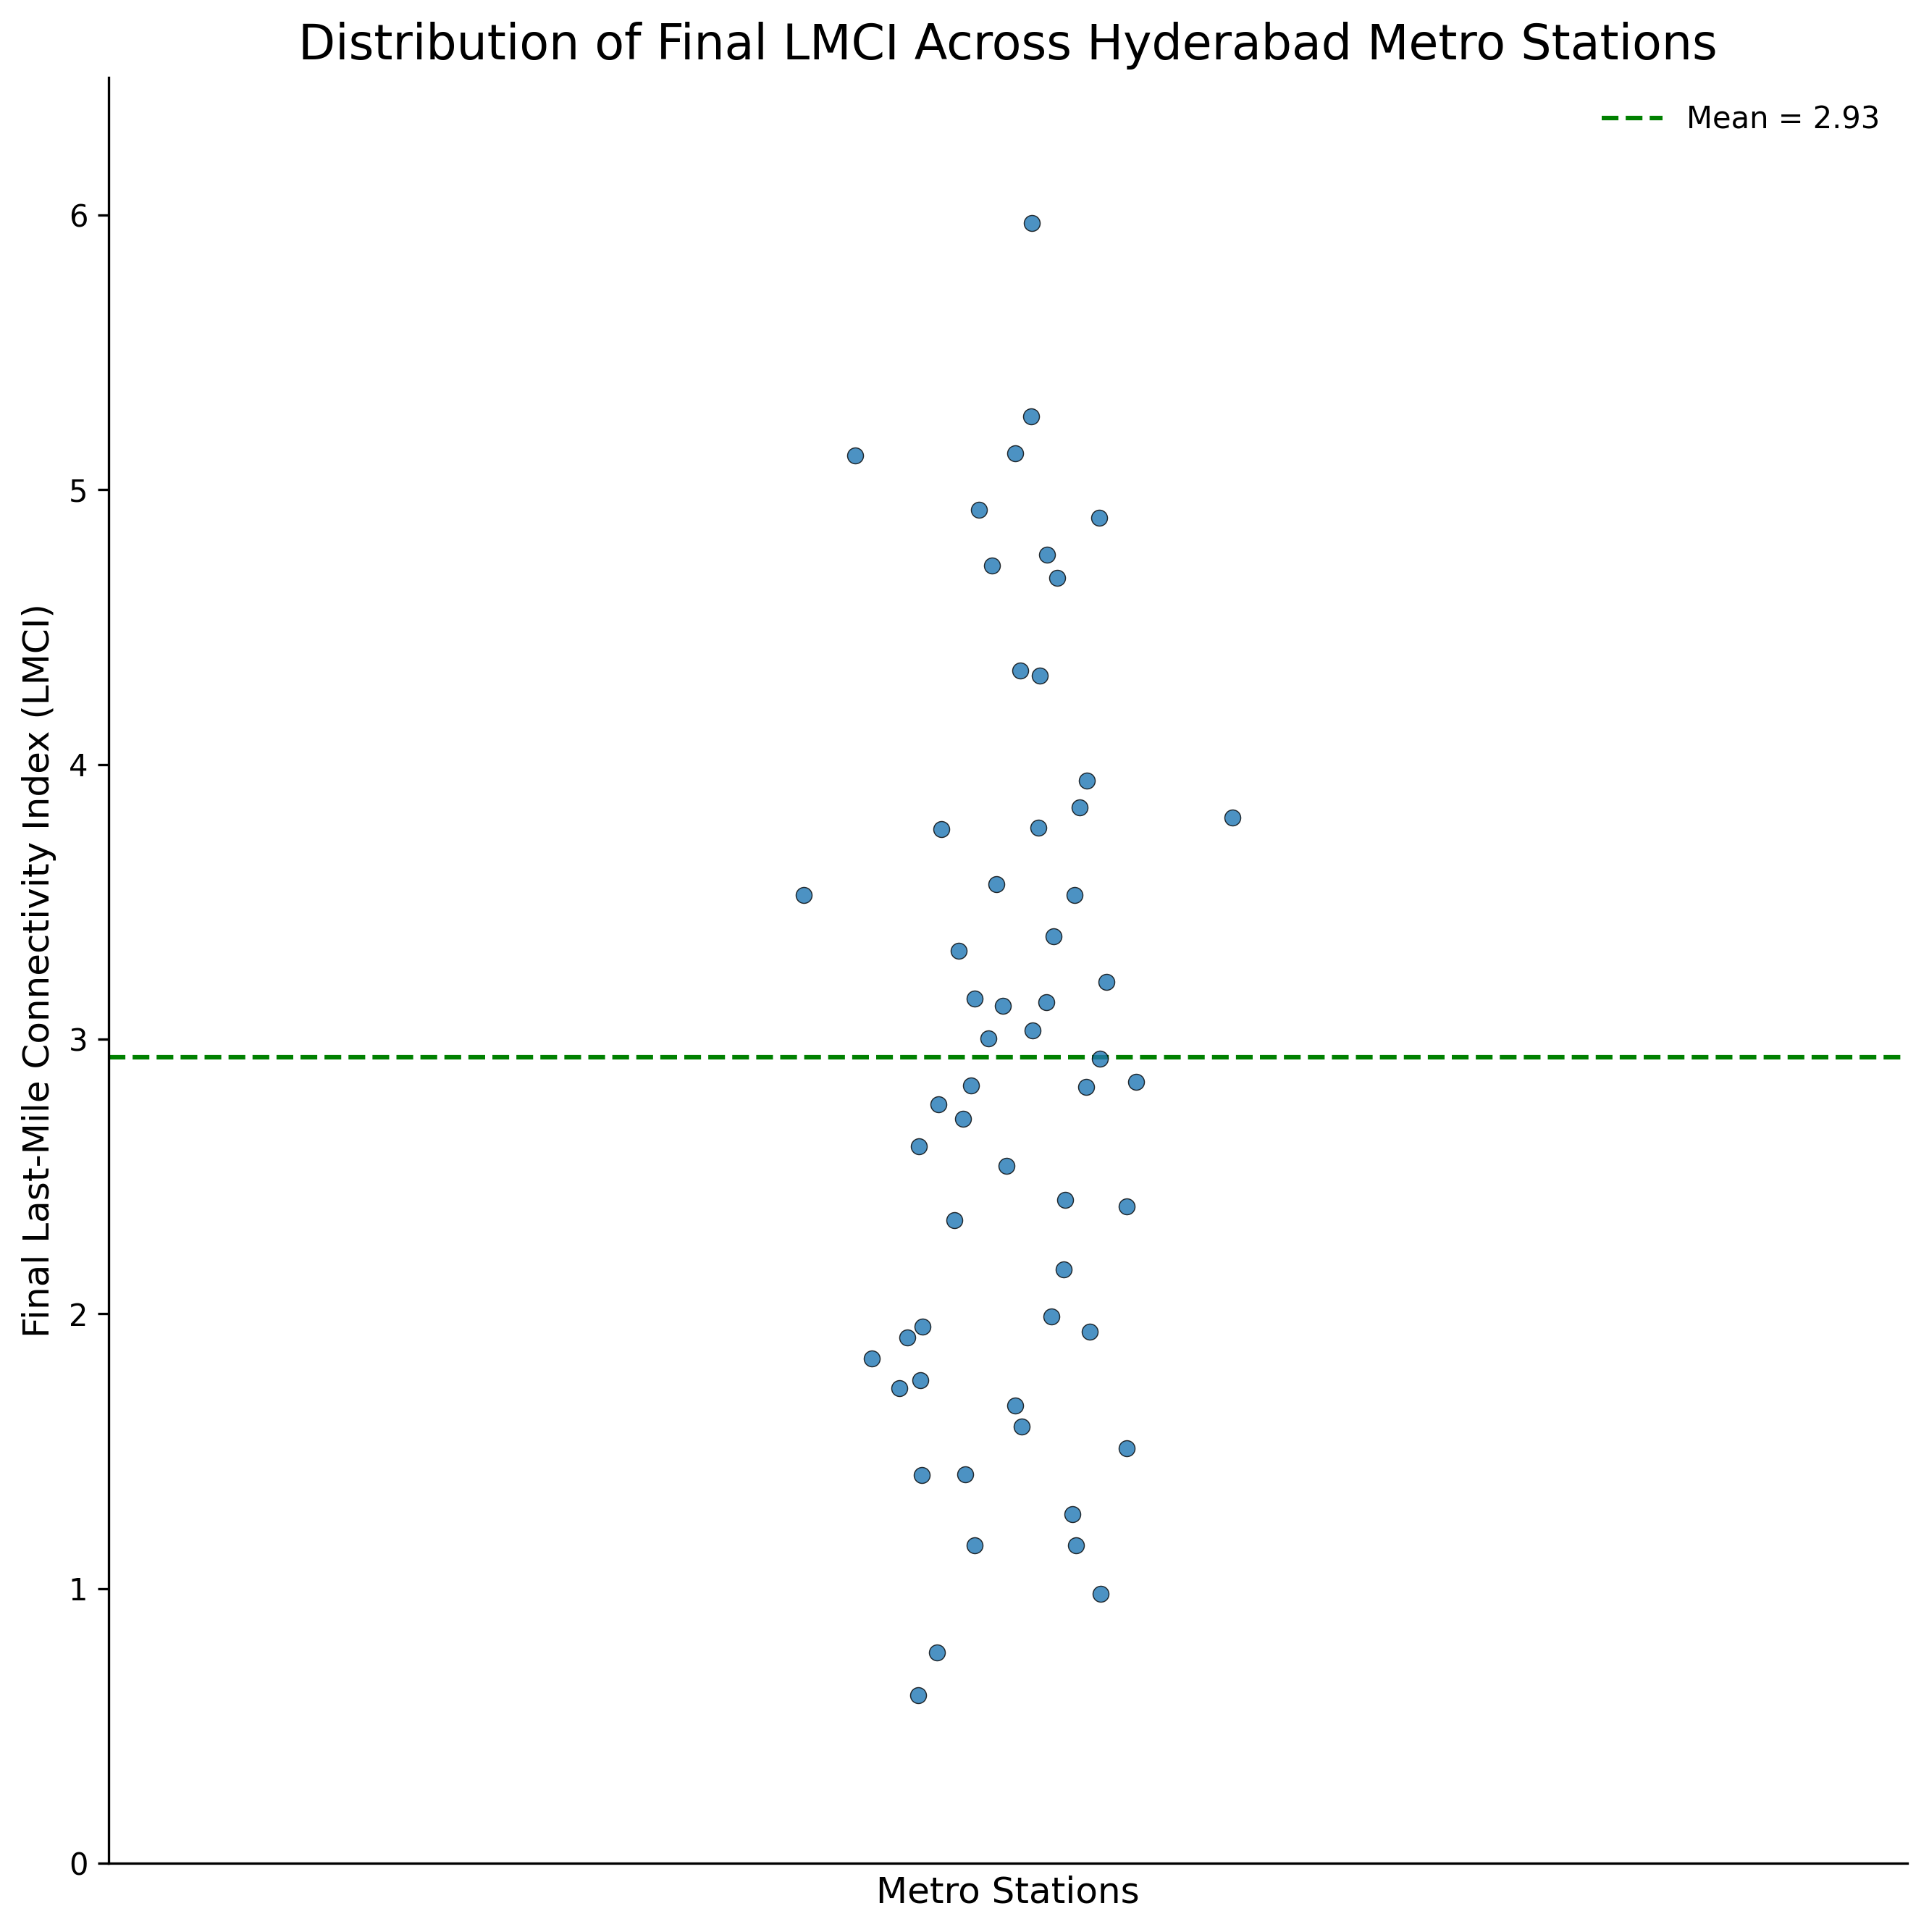
\includegraphics[width=\linewidth]{assets/plots/01_lmci_distribution.png}
\caption{[AUTHOR: WRITE CAPTION FROM ACTUAL OUTPUT - do not state a mean/range until measured]}
\label{fig:lmci_distribution}
\end{figure}

\begin{figure}[t]
\centering
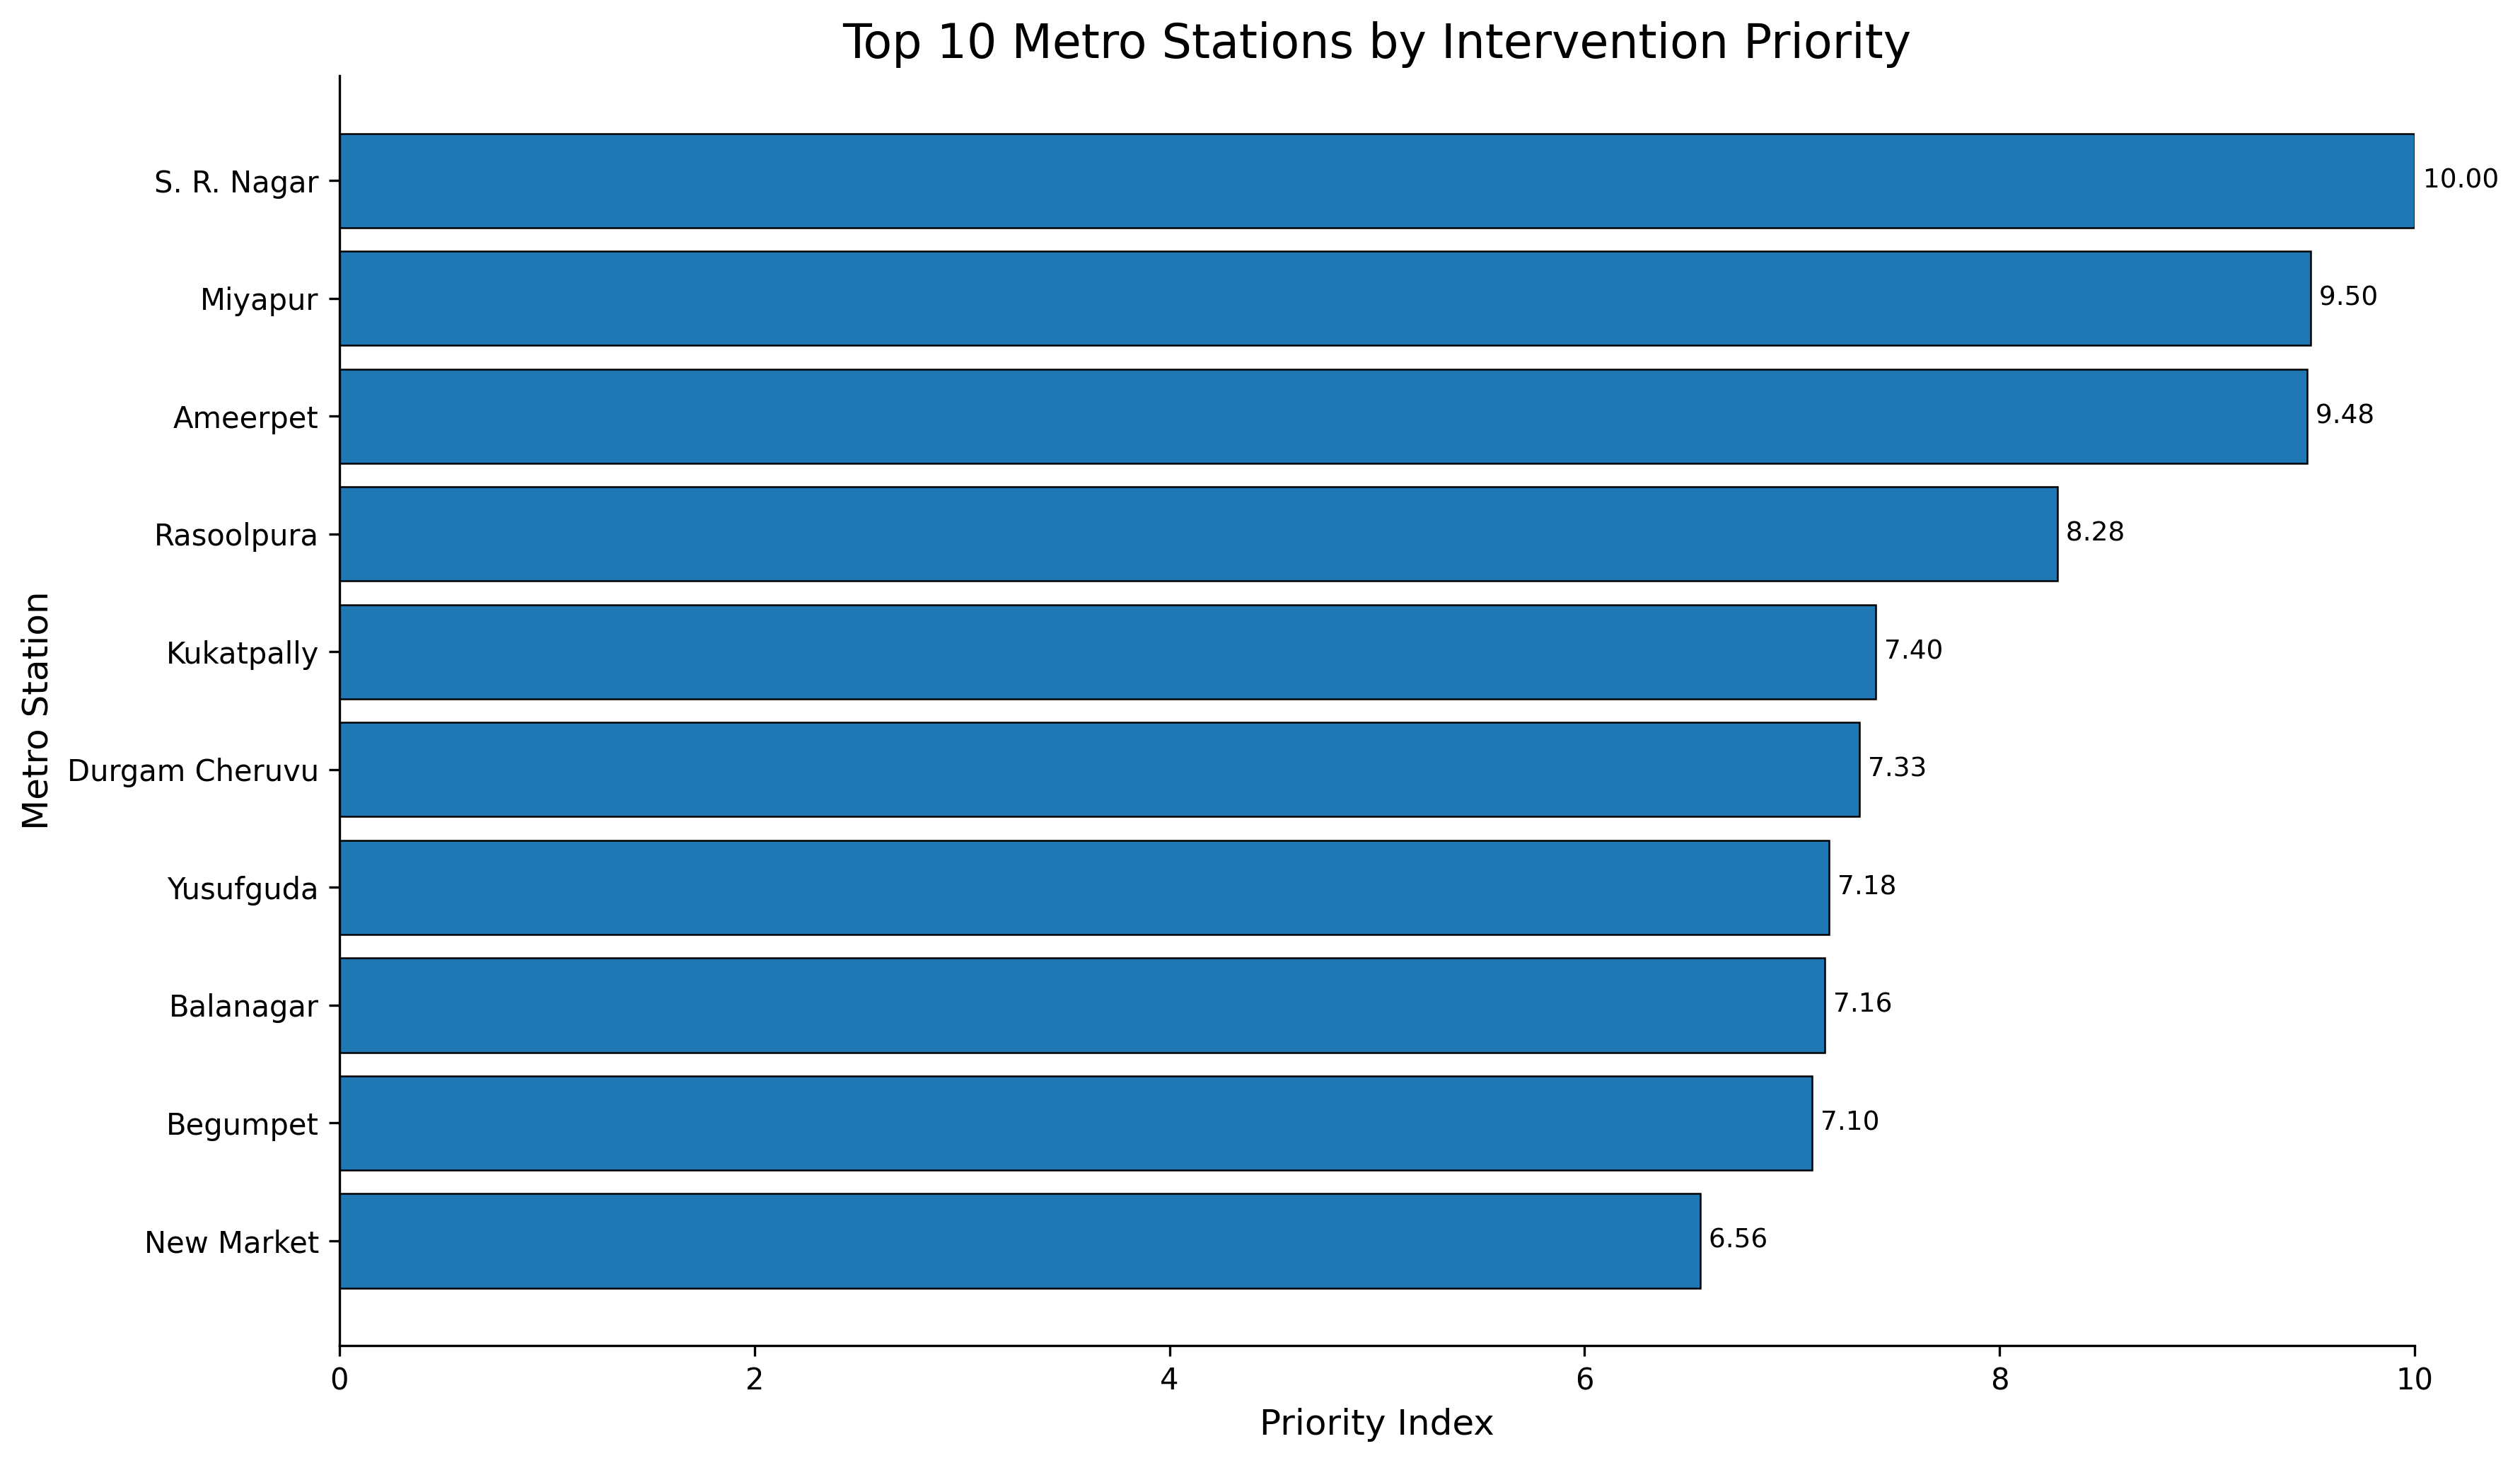
\includegraphics[width=\linewidth]{assets/plots/02_top_priority_stations.png}
\caption{[AUTHOR: WRITE CAPTION FROM ACTUAL OUTPUT]}
\label{fig:top_priority}
\end{figure}

\begin{figure}[t]
\centering
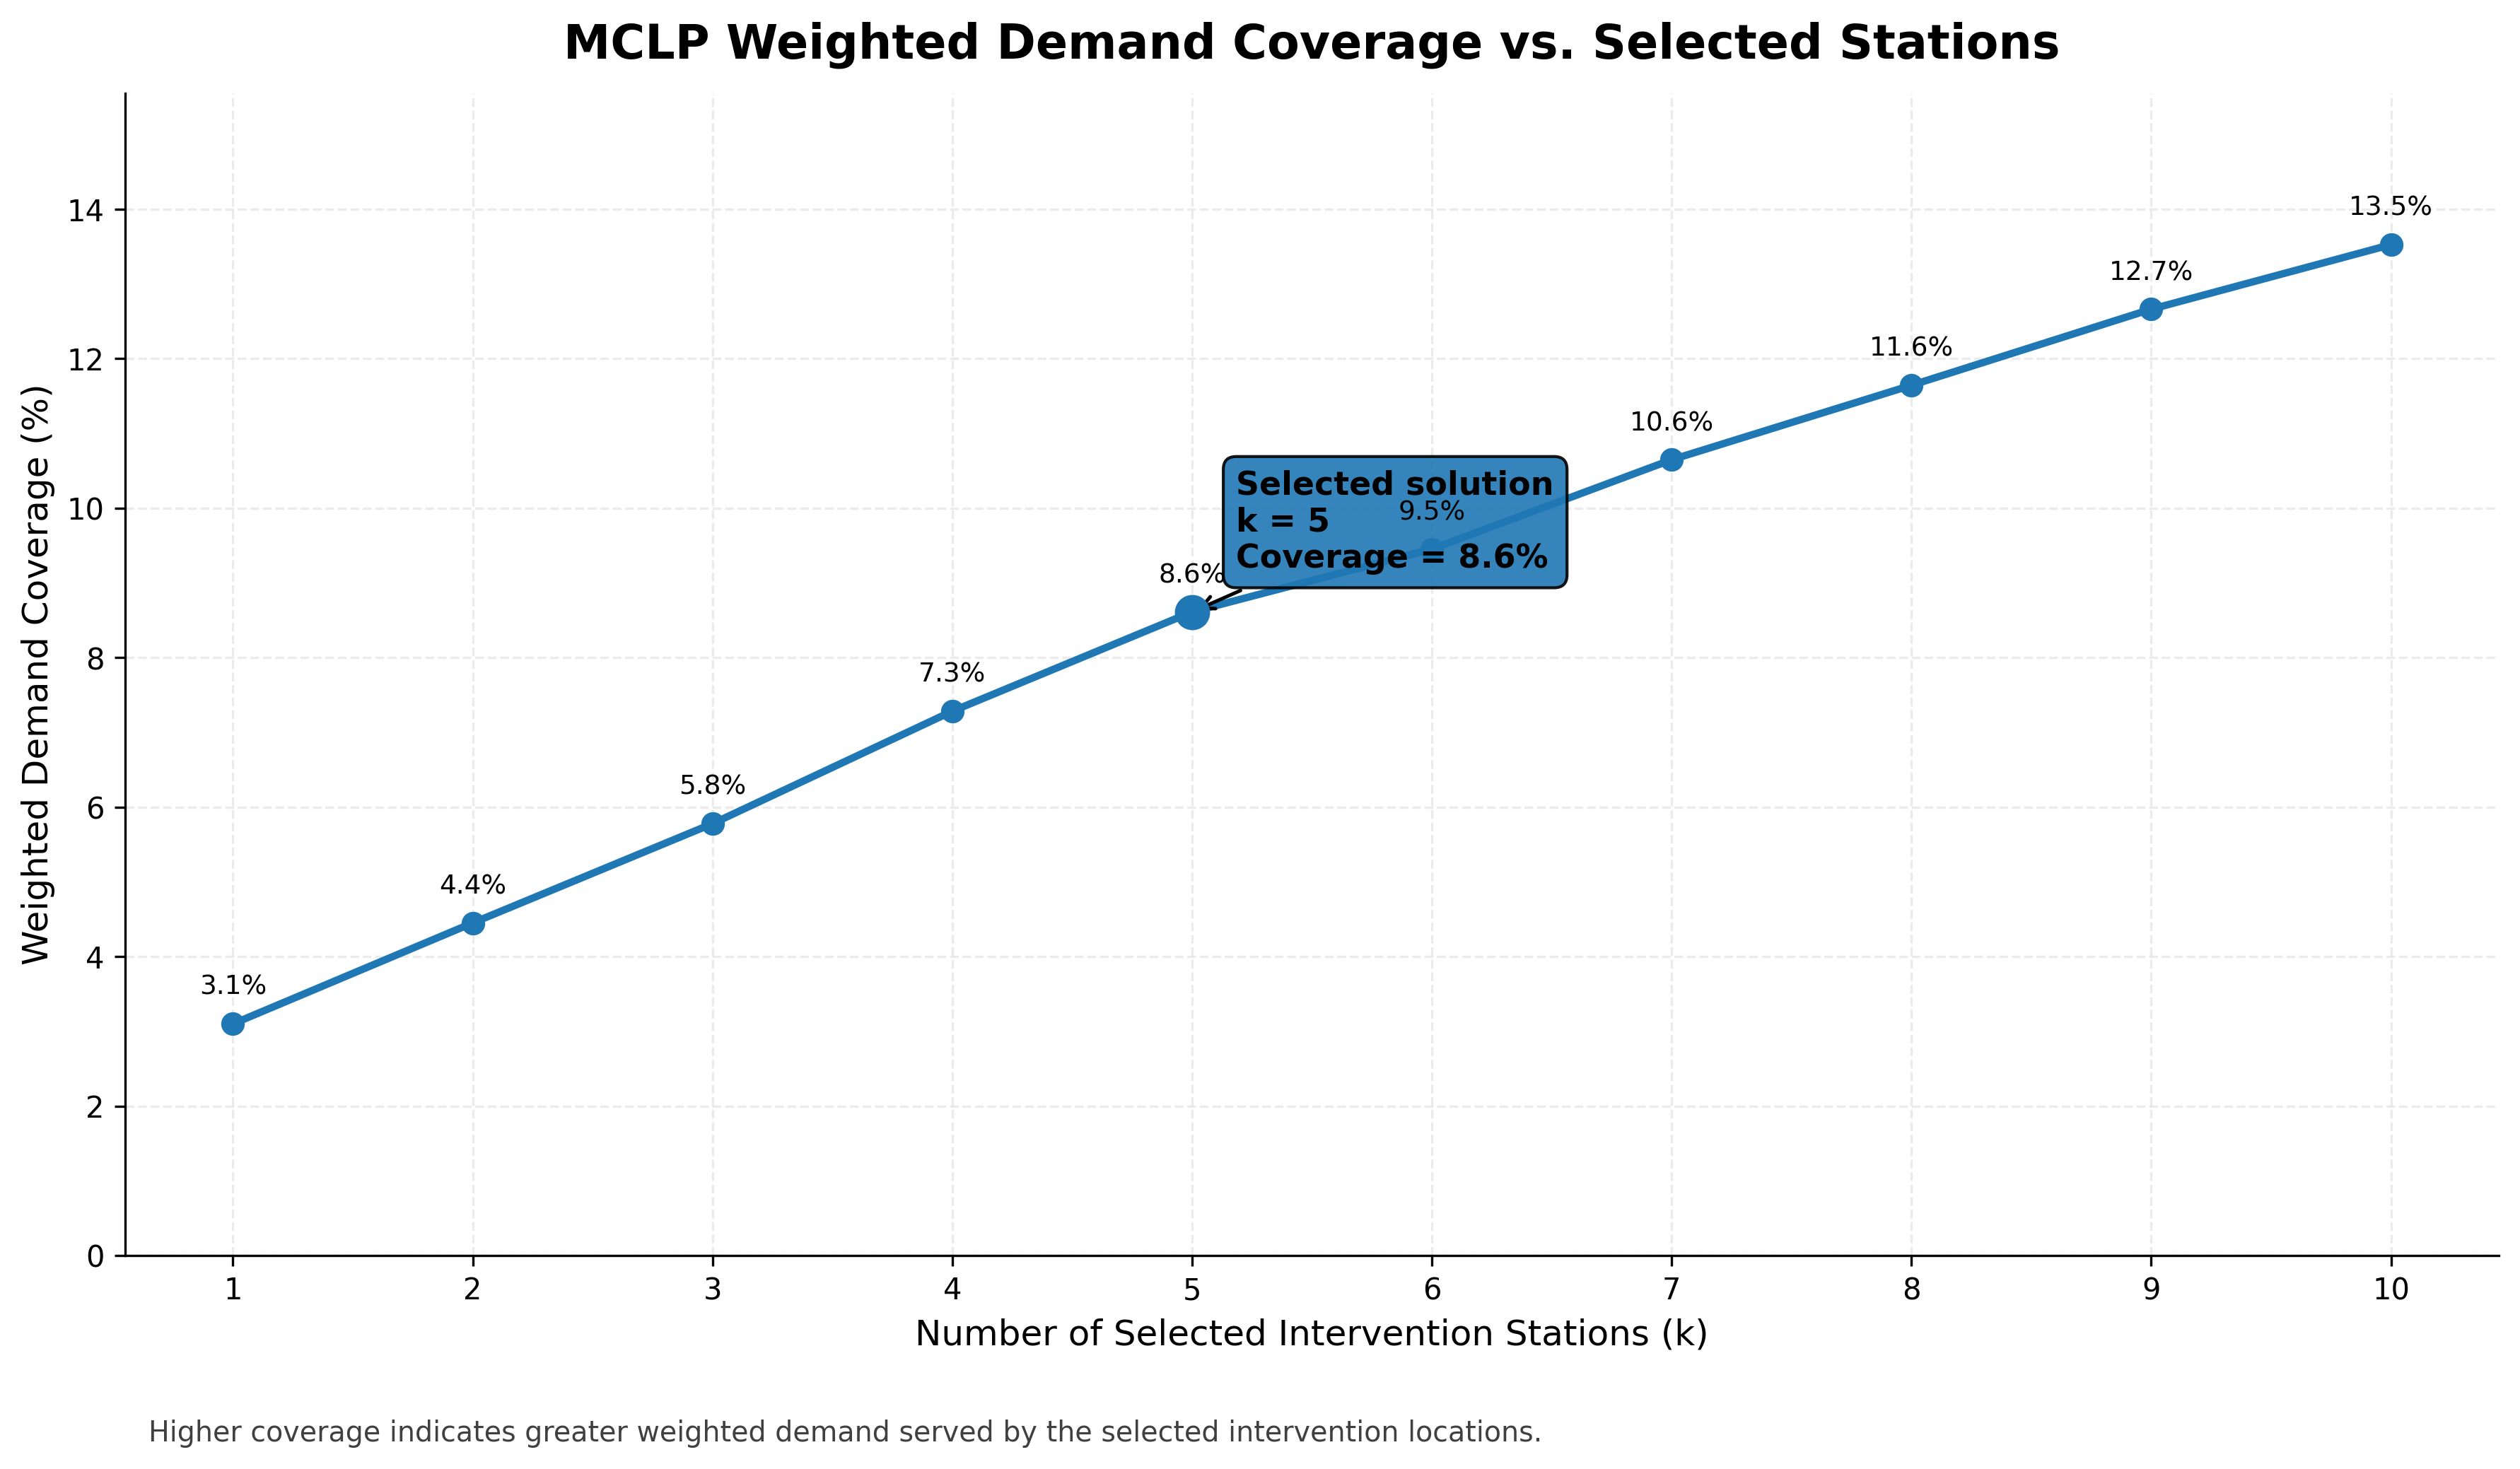
\includegraphics[width=\linewidth]{assets/plots/05_mclp_coverage_curve.png}
\caption{[AUTHOR: WRITE CAPTION FROM ACTUAL OUTPUT - MCLP is a greedy approximation, Section on Greedy MCLP Selection]}
\label{fig:mclp_coverage}
\end{figure}

\begin{figure}[t]
\centering
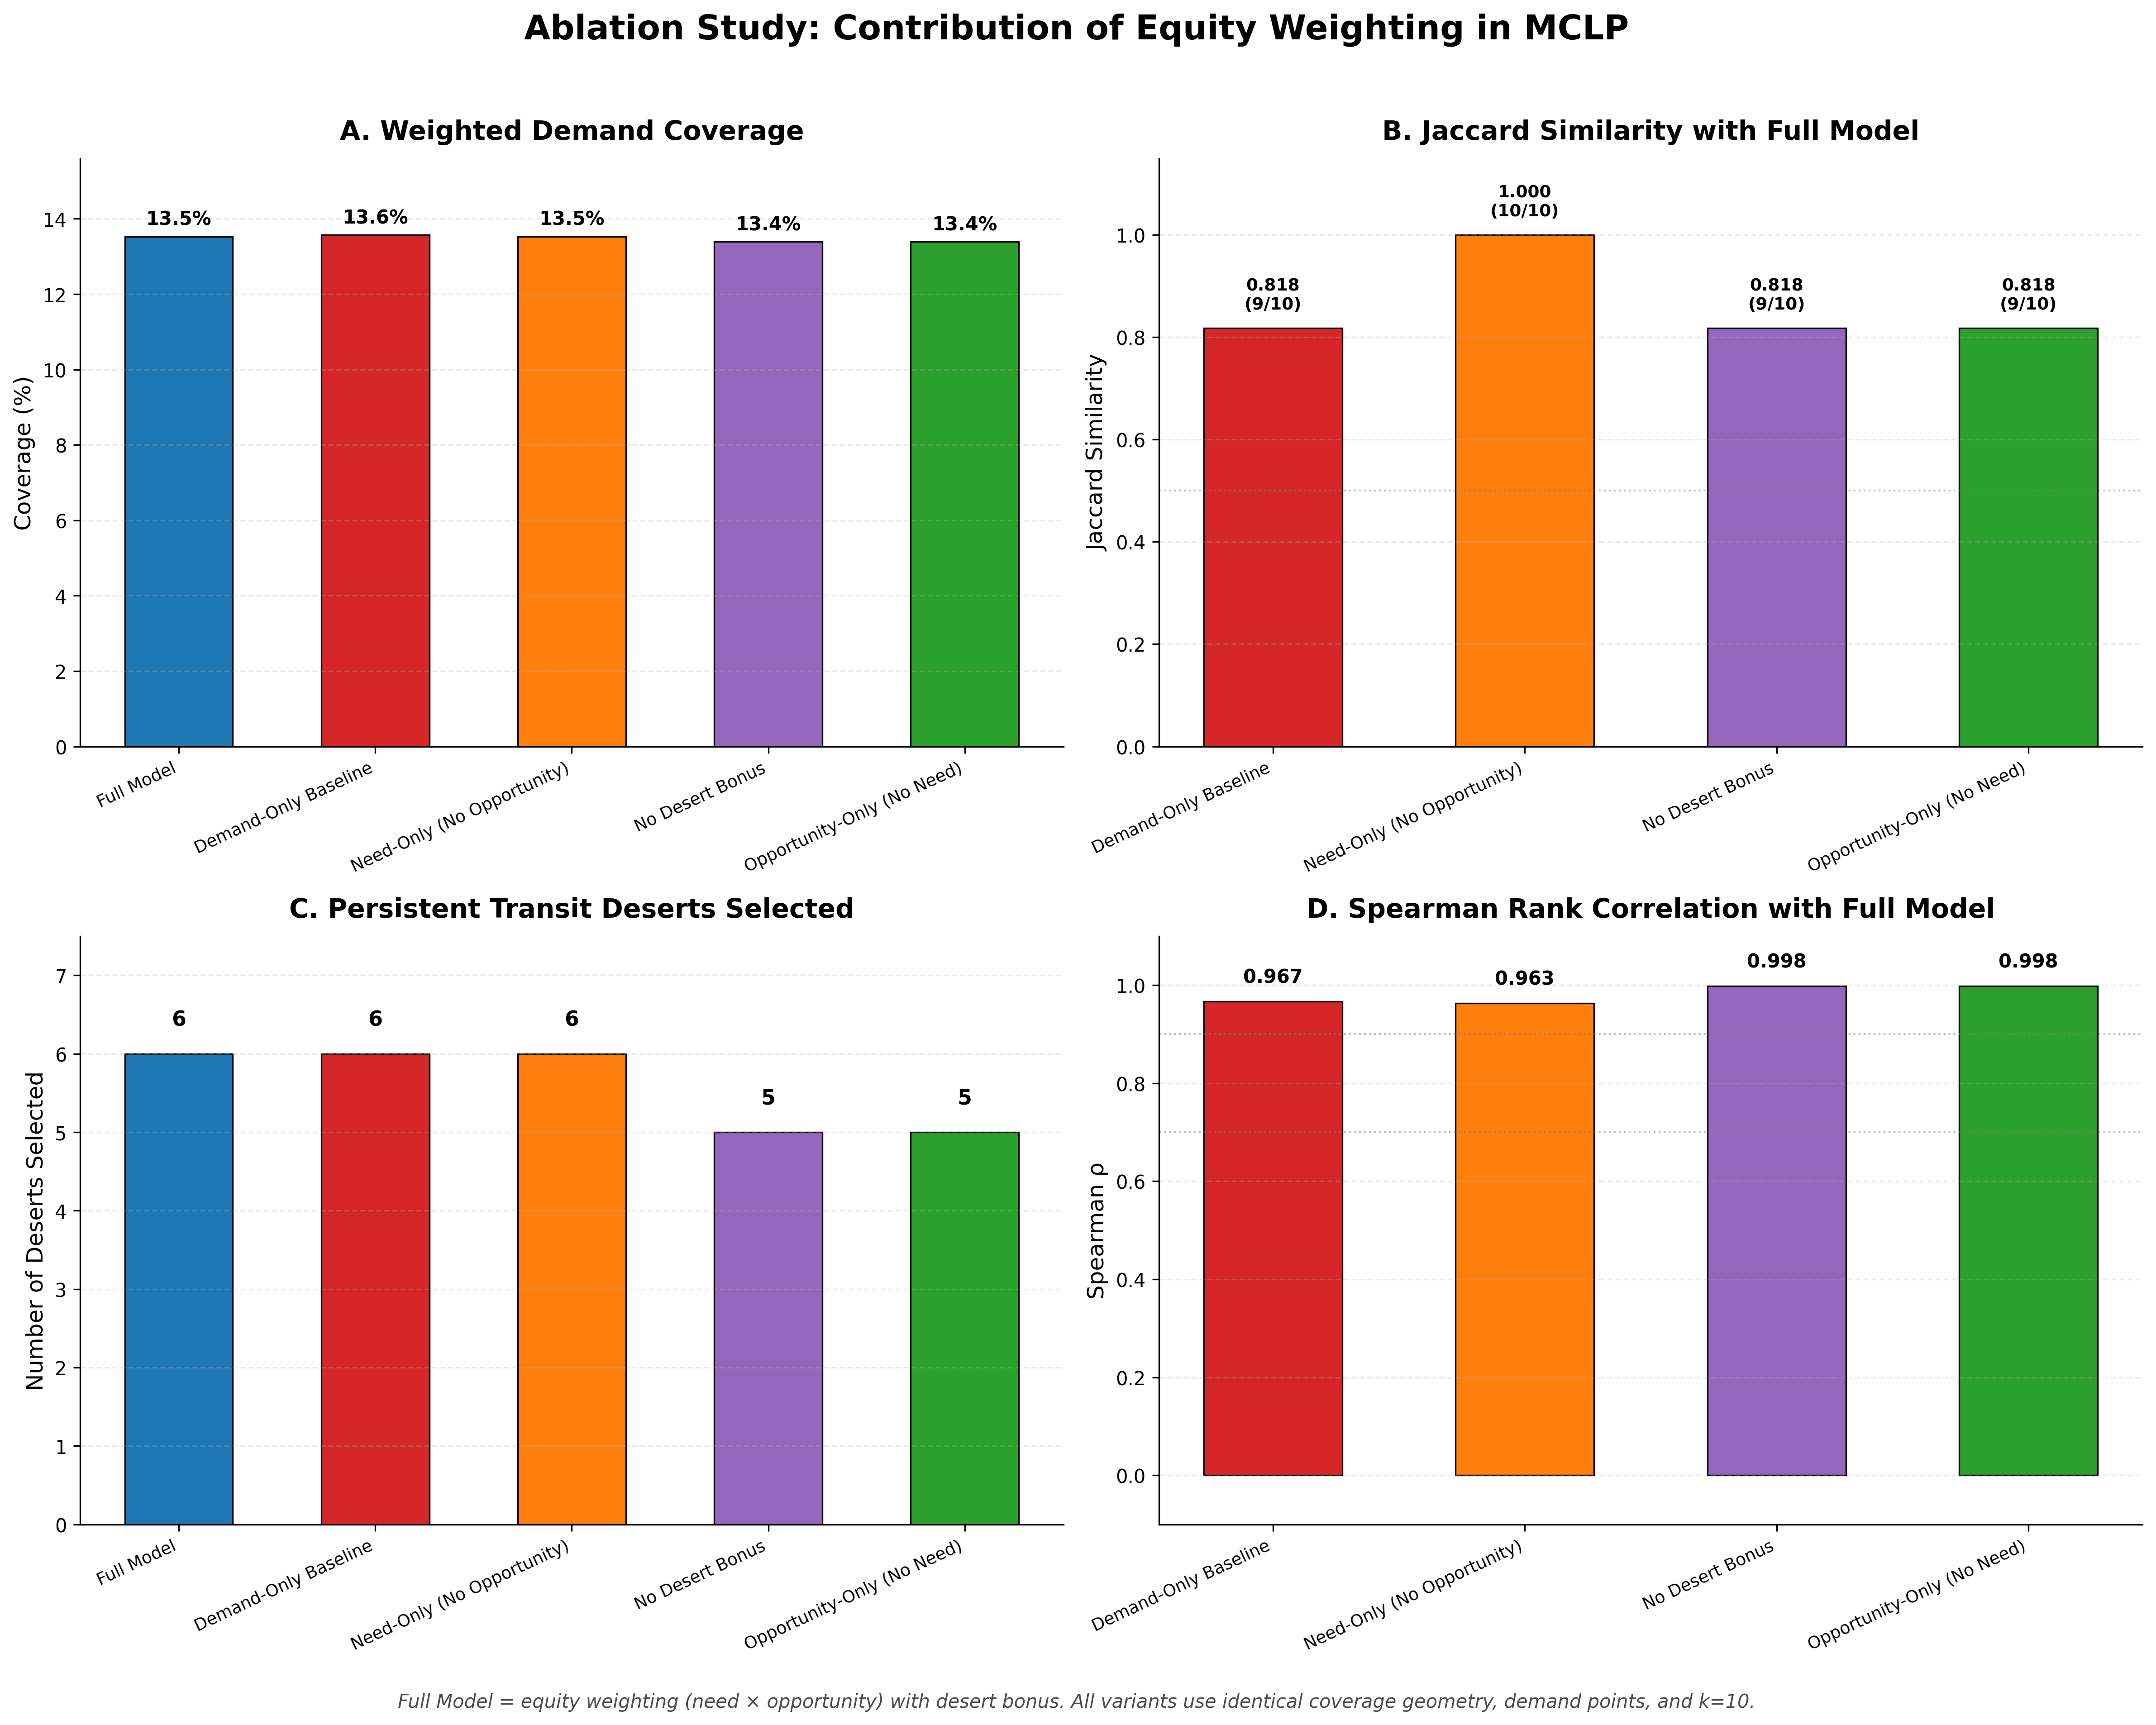
\includegraphics[width=\linewidth]{assets/plots/08_ablation_study.png}
\caption{[AUTHOR: WRITE CAPTION FROM ACTUAL OUTPUT - figure generated only if ablation data is sufficient; confirm it was produced]}
\label{fig:ablation}
\end{figure}

% Remaining figures 3,4,6,7,9,10 omitted from inline placement here for
% brevity; insert using the same \includegraphics pattern against the
% Figure Checklist above once results exist.

% ==============================================================
\section*{Implementation-to-Paper Traceability Matrix}
\begin{longtable}{p{2.0cm}p{4.0cm}p{2.6cm}p{3.0cm}}
\toprule
Code File & Function & Paper Section & Equation/Figure/Table \\
\midrule
\endhead
preprocessing.py & minmax\_norm() & Data Preprocessing & Eq.~\ref{eq:minmax} \\
preprocessing.py & haversine\_matrix() & Data Preprocessing (distance) & Eq.~\ref{eq:haversine} (unused, see observation) \\
preprocessing.py & GTFSLoader.load\_metro\_stops() & Study Area and Data & -- \\
preprocessing.py & filter\_demand\_within\_metro\_corridor() & Study Area and Data & -- \\
lmci.py & build\_multimodal\_graph() & Spatial Representation & Eq.~\ref{eq:detour} \\
lmci.py & compute\_route\_diversity() & Spatial Representation & -- \\
lmci.py & compute\_temporal\_frequency() & Temporal Service Characterization & Eq.~\ref{eq:freq} \\
lmci.py & compute\_feeder\_frequency\_from\_headways() & Temporal Service Characterization & Eq.~\ref{eq:headway} \\
lmci.py & compute\_mmts\_transfer\_penalty\_factor() & Temporal Service Characterization & Eq.~\ref{eq:mmts_penalty} \\
lmci.py & compute\_entropy\_weights() & Entropy Weighting & -- \\
lmci.py & compute\_temporal\_lmci() & LMCI (baseline/temporal) & Eq.~\ref{eq:lmci_temporal}, Eq.~\ref{eq:category} \\
lmci.py & attach\_demand\_counts() & LMCI (demand-augmented) & -- \\
lmci.py & compute\_demand\_augmented\_lmci() & LMCI (demand-augmented) & Eq.~\ref{eq:lmci_demand} \\
lmci.py & classify\_transit\_deserts() & Transit Deserts \& Priority Index & Eq.~\ref{eq:priority_score} \\
mclp.py & assign\_demand\_weights() & Greedy MCLP Selection & -- \\
mclp.py & enrich\_station\_candidates() & Greedy MCLP Selection & -- \\
mclp.py & infer\_opportunity\_score() & Greedy MCLP Selection & -- \\
mclp.py & build\_coverage\_matrix() & Greedy MCLP Selection & Eq.~\ref{eq:detour_inverse}, Fig.~\ref{fig:mclp_coverage} \\
mclp.py & greedy\_mclp() & Greedy MCLP Selection & -- \\
mclp.py & build\_candidate\_scores() & Greedy MCLP Selection & -- \\
mclp.py & run\_mclp\_ablation\_study() & Ablation Analysis & Fig.~\ref{fig:ablation} \\
mclp.py & compute\_coverage\_by\_k() & Greedy MCLP Selection & Fig.~\ref{fig:mclp_coverage} \\
scoring.py & classify\_demand\_service\_mismatch() & Demand-Service Mismatch & -- \\
scoring.py & compute\_station\_priority\_scores() & Station Priority Scoring & -- \\
scoring.py & generate\_recommendation() & Station Priority Scoring & -- \\
simulation.py & define\_intervention\_scenarios() & Intervention Scenario Simulation & Scenario table \\
simulation.py & compute\_lmci\_gain() & Intervention Scenario Simulation & Eq.~\ref{eq:lmci_gain} \\
simulation.py & compute\_impact\_multiplier() & Intervention Scenario Simulation & -- \\
simulation.py & estimate\_station\_impact() & Intervention Scenario Simulation & Eq.~\ref{eq:impact_score} \\
simulation.py & rank\_best\_interventions() & Intervention Scenario Simulation & -- \\
visualization.py & plot\_lmci\_distribution() & Experimental Results & Fig.~\ref{fig:lmci_distribution} \\
visualization.py & plot\_top\_priority\_stations() & Experimental Results & Fig.~\ref{fig:top_priority} \\
\bottomrule
\end{longtable}

\end{document}
